
\chapter{Differential Equations}

\section*{Introduction}

Up to this point, we have studied \textit{what things are}---the values of functions, the shapes of surfaces, the directions of vector fields. Now we ask a fundamentally different question: \textit{how do things change?} If we know the rate at which a population grows, can we predict its size at any future time? If we know how heat flows from hot to cold, can we predict the temperature distribution in a rod? If we know the forces on a vibrating string, can we predict its shape? These are the questions that differential equations answer.\\ \\
\noindent A differential equation is an equation involving an unknown function and its derivatives. The function is what we seek; the derivatives encode the physical law governing the system. Newton's second law \( F = ma \) is a differential equation (acceleration is the second derivative of position). Fourier's law of heat conduction is a differential equation. The wave equation, the diffusion equation, the Schr\"odinger equation---all differential equations. They are the mathematical language of physics and engineering.\\ \\
\noindent This chapter covers both \textbf{ordinary differential equations} (ODEs), where the unknown function depends on a single variable, and \textbf{partial differential equations} (PDEs), where it depends on several. For ODEs, we develop a toolkit of methods: separation of variables, integrating factors, the characteristic equation for linear equations with constant coefficients, undetermined coefficients, variation of parameters, and Laplace transforms. For PDEs, we introduce separation of variables, Fourier series, the method of characteristics, and Green's functions.\\ \\
\noindent The progression is deliberate: first-order ODEs are the simplest, requiring just one integration. Higher-order ODEs with constant coefficients reduce to algebra via the characteristic equation. Laplace transforms convert differential equations into algebraic equations wholesale. PDEs, which involve partial derivatives with respect to multiple independent variables, demand more sophisticated machinery but yield the equations that describe heat, waves, and potential theory---the phenomena we have been building toward since Chapter 1.



\newpage 



\lecture{Introduction to Differential Equations} \index{Differential Equations}

\noindent After exploring the rich landscape of multivariable calculus—from vectors to gradients, from multiple integrals to vector fields—we now turn our attention to one of mathematics' most powerful modeling tools: differential equations. While our previous studies focused on understanding rates of change and accumulation in multiple dimensions, we now ask a more fundamental question: given information about how quantities change, can we determine the quantities themselves? \\

\noindent This seemingly simple question opens the door to modeling countless real-world phenomena, from the graceful arc of a pendulum to the intricate patterns of population growth, from the flow of heat through materials to the propagation of waves through space. In each case, we begin not with the behavior itself, but with a mathematical description of how that behavior changes—a differential equation.

\begin{figure}[H]
    \centering
    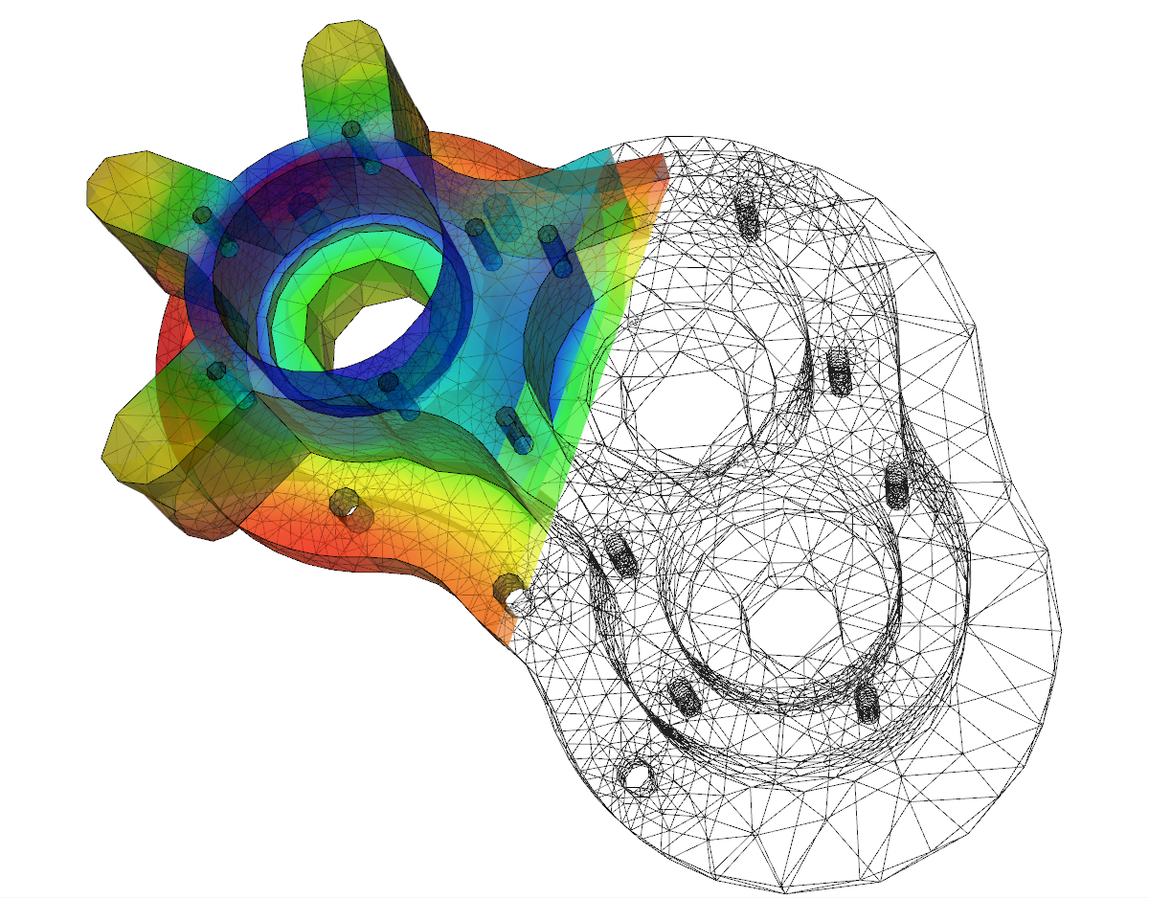
\includegraphics[width=0.55\textwidth]{chapters/chp6_pics/Elmer-pump-heatequation.png}
\caption{\textit{Visualizing the application of differential equations in finite element analysis (FEA), where partial differential equations (PDEs) model stress, strain, and deformation across complex geometries.}}
    \label{fig:fea_heat_equation}
\end{figure}

\subsection*{The Nature of Differential Equations}

\noindent A \textbf{differential equation} is an equation involving an unknown function and its derivatives. When we write:
\[
\frac{dy}{dx} = 2x
\]
we're expressing a relationship between an unknown function $y(x)$ and its derivative. The solution isn't just a number but a function—in this case, $y(x) = x^2 + C$. This represents a fundamental shift in our mathematical thinking: instead of finding values, we're finding functions that satisfy certain derivative relationships. \\

\noindent More formally, a differential equation can be written in the general form:
\[
F(x, y, y', y'', ..., y^{(n)}) = 0
\]
where $F$ is some function, $y$ is our unknown function, and $y^{(k)}$ represents the $k$th derivative of $y$. The order of a differential equation is the highest derivative that appears in it. For instance, $\frac{dy}{dx} = x^2$ is first-order, $\frac{d^2y}{dx^2} + \frac{dy}{dx} = \sin(x)$ is second-order, and $\frac{d^3y}{dx^3} - x\frac{dy}{dx} = e^x$ is third-order.

\noindent For differential equations with partial derivatives, we deal with functions of multiple variables, so the general form becomes:
\[
F(x_1, x_2, ..., x_n, u, \frac{\partial u}{\partial x_1}, \frac{\partial u}{\partial x_2}, ..., \frac{\partial^2 u}{\partial x_1^2}, \frac{\partial^2 u}{\partial x_1\partial x_2}, ...) = 0
\]
where $u = u(x_1, x_2, ..., x_n)$ is our unknown function of multiple variables, and $\frac{\partial u}{\partial x_i}$ represents partial derivatives with respect to the variable $x_i$. The order of a PDE is determined by the highest partial derivative that appears. For example:
\begin{itemize}
\item $\frac{\partial u}{\partial t} = \alpha\frac{\partial^2 u}{\partial x^2}$ (Heat equation) is second-order
\item $\frac{\partial^2 u}{\partial t^2} = c^2\frac{\partial^2 u}{\partial x^2}$ (Wave equation) is second-order
\item $\frac{\partial^2 u}{\partial x^2} + \frac{\partial^2 u}{\partial y^2} = 0$ (Laplace equation) is second-order
\end{itemize}

\subsubsection*{Origins and Formation}

\noindent Differential equations emerge naturally when we observe how quantities change in relation to each other. Consider a simple pendulum: its acceleration (second derivative of position) is proportional to its displacement, leading to:
\[
\frac{d^2\theta}{dt^2} = -\frac{g}{L}\sin(\theta)
\]
where $\theta$ is the angle from vertical, $g$ is gravitational acceleration, and $L$ is the pendulum length. How might we even begin to solve such an equation? Our calculus instincts suggest integration, but integrating both sides still leaves us with $\frac{d\theta}{dt}$ in terms of an integral of $\sin(\theta)$. This hints at the deeper complexity we'll encounter. \\

\noindent The process of forming differential equations often begins with physical insight. For instance, Newton's law of cooling states that the rate of temperature change is proportional to the temperature difference:
\[
\frac{dT}{dt} = -k(T - T_a)
\]
where $T$ is the object's temperature, $T_a$ is ambient temperature, and $k$ is a constant. Here we might have more success - notice how we could potentially separate variables with $T$ and $t$ on different sides. \\

\noindent Not all differential equations involve a single variable. Heat flow through a metal plate, as we saw, depends on position in both $x$ and $y$ directions and time $t$:
\[
\frac{\partial u}{\partial t} = \alpha\left(\frac{\partial^2 u}{\partial x^2} + \frac{\partial^2 u}{\partial y^2}\right)
\]
where $u(x,y,t)$ is temperature and $\alpha$ is thermal diffusivity. Such partial differential equations present entirely new challenges - now we're seeking functions of multiple variables! 

\exampleline
\begin{example}
A cup of hot coffee is sitting in a room of constant temperature 20°C. If the coffee's temperature drops from 90°C to 60°C in the first 10 minutes, model the coffee's temperature over time.
\begin{solution}
Let's think about how temperature changes:
\begin{enumerate}
\item First, let's understand what affects the rate of cooling:
\begin{itemize}
   \item The hotter the coffee is compared to the room, the faster it cools
   \item As the coffee gets closer to room temperature, cooling slows down
   \item The room stays at 20°C (we say it's the ambient temperature)
\end{itemize}
\item Let's translate this into mathematics:
\begin{itemize}
   \item Let $T(t)$ be the coffee's temperature at time $t$
   \item The rate of change is $\frac{dT}{dt}$
   \item The temperature difference from room temperature is $(T - 20)$
\end{itemize}
\item The rate of cooling is proportional to the temperature difference between the object and the surrounding environment. The constant in the differential equation must be negative to reflect that the object's temperature decreases over time when it is warmer than the surroundings. This yields the differential equation:
\[
\frac{dT}{dt} = -k(T - 20)
\]
\noindent This is actually known as Newton's Law of Cooling. We may find the constant $k$ using our initial conditions which will be discussed later.
\end{enumerate}

\end{solution}
\end{example}
\exampleline

\subsubsection*{Approaches to Solutions}

\noindent Solving differential equations requires a fundamentally different mindset from standard calculus. Consider first a seemingly simple ODE:
\[
\frac{dy}{dx} + y = e^x
\]
We seek a function $y(x)$ that, when substituted back, satisfies this relationship. But how? We could try guessing - since $e^x$ appears on the right, perhaps $y = Ce^x$ for some constant $C$? Or maybe we need a more systematic approach? \\

\noindent Some equations graciously yield to direct integration:
\[
\frac{dy}{dx} = x^2\sin(x)
\]
immediately suggests integrating both sides. But what about:
\[
\frac{\partial^2 u}{\partial x^2} = \frac{\partial^2 u}{\partial t^2}
\]
the famous wave equation? Integration seems less helpful here - we're dealing with partial derivatives in multiple variables. Perhaps we need a completely different strategy, like assuming solutions have a special form? \\

\noindent When analytical methods fail us, we might turn to numerical approximations. Consider discretizing our domain into small steps and approximating derivatives with finite differences:
\[
\frac{dy}{dx} \approx \frac{y(x + h) - y(x)}{h}
\]
This suggests iterative schemes that computers can implement. For PDEs, we might need to discretize in multiple dimensions, leading to systems of algebraic equations. \\

\noindent Sometimes, understanding behavior proves more valuable than finding exact solutions. For the logistic equation:
\[
\frac{dP}{dt} = rP\left(1 - \frac{P}{K}\right)
\]
we can identify equilibrium points by setting $\frac{dP}{dt} = 0$. But what about stability? How can we determine whether small perturbations grow or decay without an explicit solution? These questions lead us to qualitative theory - a powerful tool for understanding solution behavior even when exact formulas elude us. \\

\noindent We will systematically approach how to solve both ordinary and partial differential equations in the upcoming lectures.



\subsection*{Fundamental Classifications} \index{Differential Equations!Classifications}

\noindent Moving beyond basic definitions, differential equations naturally organize themselves into several fundamental categories. Each classification not only helps us understand the equation's nature but also suggests which solution methods might prove fruitful. \\

\noindent First and most fundamentally, we distinguish between ordinary and partial differential equations. An \textbf{ordinary differential equation (ODE)} \index{Ordinary Differential Equations} involves an unknown function of a single independent variable. For instance:
\[
\frac{d^2 y}{dx^2} + 3\frac{dy}{dx} + 2y = 0
\]
represents a second-order ODE. The term "ordinary" emphasizes that only ordinary derivatives appear, not partial derivatives. \\

\noindent In contrast, a \textbf{partial differential equation (PDE)} \index{Partial Differential Equations} involves an unknown function of several independent variables. The classic two-dimensional Laplace equation:
\[
\frac{\partial^2 u}{\partial x^2} + \frac{\partial^2 u}{\partial y^2} = 0
\]
appears across physics in steady-state heat conduction, electrostatics, and fluid flow. This distinction impacts not just complexity but determines which theoretical tools we can employ. \\

\noindent Another crucial distinction lies between linear and nonlinear equations. A \textbf{linear ODE of order n} \index{Linear Differential Equations} takes the form:
\[
a_n(x)\frac{d^n y}{dx^n} + a_{n-1}(x)\frac{d^{n-1}y}{dx^{n-1}} + \cdots + a_0(x)y = g(x)
\]
where $a_0, a_1, \dots, a_n, g$ are functions of $x$ alone. Linearity means $y$ and its derivatives appear to the first power, without multiplications between them and without nonlinear transformations like $\sin(y)$ or $y^2$. \\

\noindent A \textbf{nonlinear equation} \index{Nonlinear Differential Equations} violates these conditions. Terms like $(y')^2$, $y \cdot y'$, or $e^y$ indicate nonlinearity. While more challenging to solve, these equations often better capture physical reality, describing phenomena like turbulent flows or complex chemical reactions. \\

\noindent The \textbf{order} \index{Differential Equations!Order} of a differential equation is defined by its highest derivative. A third-order equation, for instance, contains terms up to $\frac{d^3y}{dx^3}$ but no higher. Higher-order equations commonly describe complex physical systems like beam deflection or wave propagation. \\

\noindent We further distinguish between homogeneous and non-homogeneous equations. A \textbf{homogeneous equation} \index{Homogeneous Differential Equations} of order $n$ has the form:
\[
a_n(x)y^{(n)} + a_{n-1}(x)y^{(n-1)} + \cdots + a_0(x)y = 0
\]
If instead the right side equals some non-zero function $g(x)$, we have a \textbf{non-homogeneous equation} \index{Non-homogeneous Differential Equations}. The homogeneous case describes free evolution, while non-homogeneous equations include external forcing. \\

\noindent Finally, for linear ODEs, we distinguish between constant and variable coefficients. In constant-coefficient equations:
\[
a_n\frac{d^n y}{dx^n} + a_{n-1}\frac{d^{n-1}y}{dx^{n-1}} + \cdots + a_0y = g(x)
\]
the coefficients $a_k$ are constants. Such equations often yield to standard solution methods. Variable-coefficient equations, where coefficients depend on $x$, typically demand more sophisticated approaches. \\

\noindent These classifications form the foundation for understanding differential equations. As we progress, we'll develop specific techniques for each type, but first recognizing an equation's category often suggests which approach might prove most fruitful.

\subsection*{Initial and Boundary Conditions} \index{Initial Conditions} \index{Boundary Conditions}

\noindent A crucial insight in differential equations is that a single equation typically has infinitely many solutions. Consider the simple equation:
\[
\frac{dy}{dx} = -2xy
\]
whose general solution we found to be $y = Ae^{-x^2}$. Each value of $A$ gives a different solution curve, collectively forming a family of solutions. \\

\begin{figure}[H]
\centering
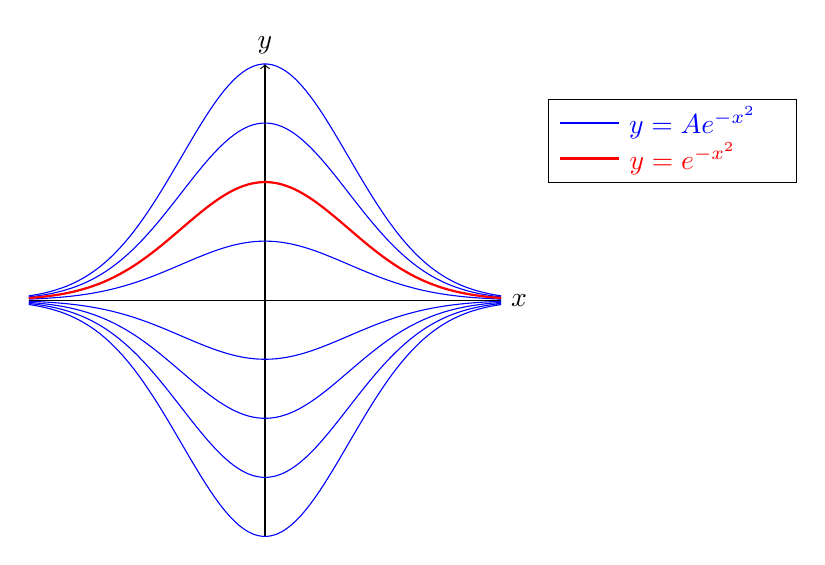
\begin{tikzpicture}[scale=1.5]
    % Draw axes
    \draw[->] (-2,0) -- (2,0) node[right] {$x$};
    \draw[->] (0,-2) -- (0,2) node[above] {$y$};
    
    % Draw solution curves for different values of A
    \foreach \a in {-2,-1.5,-1,-0.5,0.5,1,1.5,2} {
        \draw[blue, domain=-2:2,samples=100] plot (\x,{\a*exp(-\x*\x)});
    }
    
    % Draw particular solution with A=1 in red
    \draw[red,thick, domain=-2:2,samples=100] plot (\x,{exp(-\x*\x)});
    
    % Add legend
    \begin{scope}[shift={(2.5,1.5)}]
        \draw[blue] (0,0) -- (0.5,0) node[right] {$y = Ae^{-x^2}$};
        \draw[red,thick] (0,-0.3) -- (0.5,-0.3) node[right] {$y = e^{-x^2}$};
        \draw[black,thin] (-0.1,0.2) rectangle (2,-0.5);
    \end{scope}
\end{tikzpicture}
\caption{\textit{Family of solutions to $\frac{dy}{dx} = -2xy$. The blue curves show different solutions for various values of $A$, while the red curve highlights the particular solution where $A=1$.}}
\label{fig:solution_family}
\end{figure}

\noindent To single out a particular solution from this family, we need additional information. This typically comes in two forms:
\begin{enumerate}

\item \textbf{Initial Conditions} \index{Initial Value Problem} specify the value of the unknown function (and possibly its derivatives) at a single point. For example, if we require:
\[
y(0) = 3
\]
this selects the unique solution curve passing through the point $(0,3)$. As we saw earlier, this leads to $A=3$ and the particular solution $y = 3e^{-x^2}$. For higher-order equations, we might need multiple conditions at the same point:
\[
\begin{cases} 
y(0) = 1 \\ 
y'(0) = 0 
\end{cases}
\]

\item \textbf{Boundary Conditions} \index{Boundary Value Problem} specify values at multiple points. For instance:
\[
y(0) = 0, \quad y(1) = 2
\]
requires our solution to pass through both $(0,0)$ and $(1,2)$. This type of condition often appears in physical problems like heat distribution or beam deflection where we know values at the endpoints of our domain.
\end{enumerate}

\noindent An equation together with sufficient conditions forms either an \textbf{Initial Value Problem (IVP)} or \textbf{Boundary Value Problem (BVP)}, depending on the type of conditions specified. The distinction is more than technical—the methods we use to solve these problems and even the nature of their solutions can differ dramatically. For instance:

\begin{enumerate}
   \item IVPs typically have unique solutions that can be ``evolved" forward from the initial condition
   \item BVPs might have multiple solutions, no solutions, or unique solutions depending on the boundary conditions
   \item Higher-order equations require correspondingly more conditions for uniqueness
\end{enumerate}

\noindent The geometric interpretation is illuminating: initial/boundary conditions effectively ``select" one curve from the infinite family of possible solutions. This idea of a family of solutions punctuated by particular solutions meeting specific conditions will recur throughout our study of differential equations, helping us understand both the general behavior of solutions and the role of additional conditions in selecting specific ones. Note, that the order of the equation must require that many conditions in order to fully produce a particular solution.

\exampleline
\begin{example}
Consider the ordinary differential equation:
\[
\frac{dy}{dx} = -2xy
\]
with initial condition $y(0) = 3$. Let's carefully examine how we might solve this equation.

\begin{solution}
Let's think about how to solve this step by step. We have a first order differential equation where we can separate all terms with $y$ on one side and all terms with $x$ on the other. \\

\noindent First, let's rearrange the equation to group $y$ terms and $x$ terms:
\[
\frac{dy}{y} = -2x\,dx
\]

\noindent Now we can integrate both sides. On the left, we recognize $\frac{dy}{y}$ as the derivative of $\ln|y|$:
\begin{align*}
\int \frac{dy}{y} &= \int -2x\,dx \\
\ln|y| &= -x^2 + C
\end{align*}

\noindent To solve for $y$, we exponentiate both sides:
\[
|y| = e^{-x^2 + C} = e^{-x^2}e^C = Ae^{-x^2}
\]
where $A = e^C$ is some positive constant. Since $A$ can be positive or negative (thanks to the absolute value), our general solution is:
\[
y = Ae^{-x^2}
\]

\noindent Now we can use our initial condition $y(0) = 3$ to find $A$:
\begin{align*}
3 &= Ae^{-0^2} \\
3 &= A \cdot 1 \\
A &= 3
\end{align*}

\noindent Therefore, our particular solution is:
\[
y = 3e^{-x^2}
\]
\end{solution}
\end{example}
\exampleline
\subsection*{Verification of Solutions} \index{Verification of Solutions}

\noindent Verifying solutions to differential equations is a critical step in ensuring the accuracy of our work. While finding solutions often requires creativity and problem-solving, verification is a systematic process that provides confidence in the correctness of the result. This process can be broken into clear steps for clarity and consistency. \\

\noindent First, we compute the necessary derivatives of the proposed solution. These derivatives are the building blocks we need to substitute back into the original differential equation. Next, by substituting the solution and its derivatives into the equation, we check whether the left-hand side equals the right-hand side. If this identity holds true, it confirms that the solution satisfies the differential equation itself. Finally, we verify any additional conditions, such as initial or boundary values, to ensure the solution fully satisfies all requirements of the problem. \\

\noindent Consider a simple example. To verify that $y(x) = x^2 + 1$ solves $\frac{dy}{dx} = 2x$:
\begin{align*}
\text{Given solution: } & y(x) = x^2 + 1 \\
\text{Compute derivative: } & \frac{dy}{dx} = 2x \\
\text{Original equation: } & \frac{dy}{dx} = 2x \\
\text{Therefore: } & 2x = 2x \quad \text{(Identity verified)}
\end{align*}

\noindent For higher-order equations, we must check more derivatives. Consider verifying that $y(x) = e^{2x}$ solves $\frac{d^2y}{dx^2} - 4y = 0$:
\begin{align*}
\text{Given: } & y = e^{2x} \\
\text{First derivative: } & \frac{dy}{dx} = 2e^{2x} \\
\text{Second derivative: } & \frac{d^2y}{dx^2} = 4e^{2x} \\
\text{Substitute: } & 4e^{2x} - 4(e^{2x}) = 0 \\
\text{Simplify: } & 0 = 0 \quad \text{(Identity verified)}
\end{align*}

\noindent For partial differential equations, we follow the same principle but must compute partial derivatives. To verify $u(x,t) = e^{-\pi^2t}\sin(\pi x)$ solves the heat equation $\frac{\partial u}{\partial t} = \frac{\partial^2 u}{\partial x^2}$:
\begin{align*}
\text{Given: } & u = e^{-\pi^2t}\sin(\pi x) \\
\text{Time derivative: } & \frac{\partial u}{\partial t} = -\pi^2e^{-\pi^2t}\sin(\pi x) \\
\text{Space derivative: } & \frac{\partial u}{\partial x} = \pi e^{-\pi^2t}\cos(\pi x) \\
\text{Second space derivative: } & \frac{\partial^2 u}{\partial x^2} = -\pi^2e^{-\pi^2t}\sin(\pi x) \\
\text{Original equation: } & \frac{\partial u}{\partial t} = \frac{\partial^2 u}{\partial x^2} \\
\text{Substitute: } & -\pi^2e^{-\pi^2t}\sin(\pi x) = -\pi^2e^{-\pi^2t}\sin(\pi x) \\
\text{Therefore: } & \text{Identity verified}
\end{align*}

\noindent Important considerations when verifying solutions:
\begin{enumerate}
   \item Check \textit{all} conditions - not just the differential equation but also initial/boundary conditions
   \item Pay attention to domains - where is the solution valid?
   \item Watch for hidden assumptions - are we dividing by zero anywhere?
   \item Use verification as a sanity check - does the solution make physical sense?
\end{enumerate}

\noindent Verification plays a crucial role in solving differential equations. It helps catch computational errors, validates the solution techniques, and builds confidence in our methods. Moreover, it fosters intuition about the behavior of solutions, enhancing our understanding of the problem. \\

\exampleline
\begin{example}
Verify that $y = x + \sum_{n=1}^{\infty} \frac{y^n}{n}$ is a solution to $y' = 1-\frac{1}{y}$. Discuss any insights about this solution.

\begin{solution}
Let's follow our verification steps:

\item Compute derivatives
  \begin{itemize}
     \item We have an implicit equation requiring implicit differentiation
     \item Start with: $y = x + \sum_{n=1}^{\infty} \frac{y^n}{n}$
     \item Differentiate both sides:
       \begin{align*}
       \frac{d}{dx}(y) &= \frac{d}{dx}\left(x + \sum_{n=1}^{\infty} \frac{y^n}{n}\right) \\
       y' &= 1 + \sum_{n=1}^{\infty} \frac{ny^{n-1}}{n}y' \\
       &= 1 + y'\sum_{n=1}^{\infty} y^{n-1}
       \end{align*}
  \end{itemize}

\item Manipulate to standard form
  \begin{itemize}
     \item Recognize $\sum_{n=1}^{\infty} y^{n-1}$ as geometric series $\frac{1}{1-y}$ for $|y| < 1$
     \item Therefore: $y' = 1 + y'\frac{1}{1-y}$
     \item Solve for $y'$:
       \begin{align*}
       y'\left(1 - \frac{1}{1-y}\right) &= 1 \\
       y'\left(\frac{-y}{1-y}\right) &= 1 \\
       y' &= 1 - \frac{1}{y}
       \end{align*}
  \end{itemize}

\item Additional insights
  \begin{itemize}
     \item The sum $\sum_{n=1}^{\infty} \frac{y^n}{n}$ is the Taylor series of $-\ln(1-y)$
     \item Solution can be written more compactly: $y = x - \ln(1-y)$
     \item Valid only for $|y| < 1$ due to series convergence
  \end{itemize}
\end{solution}
\end{example}
\exampleline

\newpage

\lecture{First-Order Ordinary Differential Equations} \index{First-Order ODEs}

\noindent Having established the fundamental nature and classification of differential equations, we now delve into our first systematic study of solution techniques for first-order ordinary differential equations. These equations, while seemingly simple in form, encompass a rich variety of mathematical structures and solution methods that form the foundation for understanding more complex differential equations. \\

\noindent A \textbf{first-order ordinary differential equation} can be written in the general form:
\[
F(x, y, y') = 0
\]
where $F$ is some function of the independent variable $x$, the dependent variable $y$, and its first derivative $y'$. More commonly, we encounter these equations in solved form:
\[
\frac{dy}{dx} = f(x,y)
\]
where $f(x,y)$ represents the relationship between the variables and the rate of change. \\

\noindent The designation ``first-order" refers to the highest derivative present in the equation - in this case, only the first derivative appears. This seemingly simple characteristic has profound implications. Unlike higher-order equations which may require multiple conditions to specify a unique solution, a first-order equation requires only a single initial condition of the form $y(x_0) = y_0$ to determine a unique solution (when one exists). \\

\noindent When studying first-order equations, we often encounter them in various standard forms, each suggesting its own solution strategy. For instance, when $f(x,y)$ can be written as a product of functions of $x$ and $y$ separately, we have a separable equation. When $f(x,y)$ is linear in $y$, we have a linear first-order equation. These special forms, which we will study in detail, provide scaffolding for understanding more general cases. \\

\noindent The existence and uniqueness of solutions to first-order equations is governed by the fundamental theorem for first-order ODEs: if $f(x,y)$ and $\frac{\partial f}{\partial y}$ are continuous in some rectangle containing an initial point $(x_0, y_0)$, then there exists a unique solution to the initial value problem in some interval containing $x_0$. This theorem provides theoretical foundation for our solution methods and helps us understand when and where we can expect solutions to exist.

\subsection*{Separation of Variables} \index{Separation of Variables}

\noindent The method of separation of variables represents our first and easiest systematic approach to solving differential equations. This technique applies when we can rewrite our equation in the form:
\[
\frac{dy}{dx} = f(x)g(y)
\]
where $f$ depends only on $x$ and $g$ depends only on $y$. The key insight is to rearrange terms so that all $y$-dependent terms are on one side and all $x$-dependent terms are on the other. This will always be your go to first visual check when trying to solve an ODE.\\

\noindent More formally, we rewrite the equation as:
\[
\frac{1}{g(y)}dy = f(x)dx
\]
This transformation allows us to integrate both sides independently:
\[
\int \frac{1}{g(y)}dy = \int f(x)dx + C
\]

\noindent The resulting equation implicitly defines $y$ as a function of $x$. In fortunate cases, we can solve explicitly for $y$, though often the solution remains in implicit form. This method's elegance lies in its reduction of a differential equation to algebraic manipulation and integration. This method obviously extends for cases of higher order derivatives which will be addressed later in this chapter.\\

\noindent Several theoretical considerations deserve attention:
\begin{enumerate}
    \item The method assumes $g(y) \neq 0$. Points where $g(y) = 0$ may yield additional solutions.
    \item The integration introduces a constant $C$, generating a family of solutions. Both integrations of $g$ and $f$ produce an arbitrary constant, but we can just combine them to form one arbitrary constant instead of two -- A fact that will be used frequently in the solving of DEs.
    \item Solutions may exist only on intervals where both $f$ and $g$ are continuous.
\end{enumerate}

\noindent We have already reasoned our way through one separable ODE in the last lecture. Let's try one that is not so obvious:

\exampleline
\begin{example}
Solve the differential equation:
\[
\frac{dy}{dx} = \frac{xy+3x+2y+6}{xy+x+y+1}
\]

\begin{solution}
Let's solve this step by step:
\begin{enumerate}
\item First, notice that both numerator and denominator can be factored through grouping:
   \begin{align*}
   xy+3x+2y+6 &= x(y+3)+2(y+3) \\
   &= (x+2)(y+3)
   \end{align*}
   And similarly:
   \begin{align*}
   xy+x+y+1 &= x(y+1)+1(y+1) \\
   &= (x+1)(y+1)
   \end{align*}

\item Our differential equation becomes:
   \[
   \frac{dy}{dx} = \frac{(x+2)(y+3)}{(x+1)(y+1)}
   \]

\item To separate variables, multiply both sides by $dx$ and rearrange:
   \[
   \frac{y+1}{y+3}\,dy = \frac{x+2}{x+1}\,dx
   \]

\item To integrate, first perform partial fractions on each side:
   \begin{align*}
   \frac{y+1}{y+3} &= 1 - \frac{2}{y+3} \\
   \frac{x+2}{x+1} &= 1 + \frac{1}{x+1}
   \end{align*}

\item Our equation becomes:
   \[
   \int \left(1 - \frac{2}{y+3}\right)dy = \int \left(1 + \frac{1}{x+1}\right)dx
   \]

\item Integrate both sides:
   \begin{align*}
   y - 2\ln|y+3| + C_1 &= x + \ln|x+1| + C_2
   \end{align*}

\item Combining constants, our general solution is:
   \[
   y - 2\ln|y+3| = x + \ln|x+1| + C, x \neq -1, y \neq -3
   \]
\end{enumerate}
\end{solution}
\end{example}
\exampleline


\subsection*{Linear First-Order Equations} \index{Linear First-Order ODEs}

\noindent A \textbf{linear first-order ODE} takes the standard form:
\[
\frac{dy}{dx} + P(x)y = Q(x)
\]
where $P(x)$ and $Q(x)$ are continuous functions. The linearity refers to the fact that $y$ and its derivative appear to the first power only, with no products between them and no nonlinear functions of $y$. When $Q(x) = 0$, we call the equation homogeneous; otherwise, it's non-homogeneous. This distinction plays a crucial role in both the theory and solution methods. \\

\noindent Any first-order linear equation can be written in this standard form through algebraic manipulation. For instance, equations like:
\[
\frac{dy}{dx} = ay + b \quad \text{or} \quad x\frac{dy}{dx} - 2y = x^3
\]
can be rewritten in standard form by collecting terms and dividing appropriately. This standardization is more than cosmetic—it reveals the underlying structure and suggests solution strategies. \\

\noindent The solution method involves an elegant technique called the \textbf{integrating factor} \index{Integrating Factor}. The key insight is that our equation almost looks like the product rule for derivatives (we're aiming for $(\mu y)' = \mu'y + \mu y')$, but not quite. If we could somehow make the left side into a perfect differential—that is, find a function $\mu(x)$ that when multiplied through makes the left side exactly the derivative of a product $\frac{d}{dx}[\mu(x)y]$—then we could solve by simple integration. With this motivation in mind, we multiply both sides by a carefully chosen function $\mu(x)$ that makes the left side the derivative of a product:
\[
\mu(x)\frac{dy}{dx} + \mu(x)P(x)y = \mu(x)Q(x)
\]

\noindent The magic of this method lies in choosing $\mu(x)$ to make the left side a perfect differential. The integrating factor $\mu(x)$ must satisfy:
\[
\frac{d}{dx}[\mu(x)y] = \mu(x)\frac{dy}{dx} + \mu'(x)y
\]
For this to equal our left side, we require:
\[
\mu'(x)y = \mu(x)P(x)y
\]
Therefore:
\[
\mu'(x) = \mu(x)P(x)
\]

\noindent This first-order separable equation for $\mu$ yields:
\[
\frac{d\mu}{\mu} = P(x)dx
\]
Integration gives us:
\[
\mu(x) = e^{\int P(x)dx}
\]

\noindent After multiplication by $\mu(x)$, our equation takes the elegant form:
\[
\frac{d}{dx}[\mu(x)y] = \mu(x)Q(x)
\]
Integration yields the general solution:
\[
y = \frac{1}{\mu(x)}\left[\int \mu(x)Q(x)dx + C\right]
\]

\noindent Several theoretical aspects deserve attention:

\begin{enumerate}
    \item The integrating factor is not unique—any constant multiple of $\mu(x)$ also works.
    \item The solution process naturally splits into finding a complementary function (solution to homogeneous equation) and a particular integral.
    \item The method always works when $P(x)$ and $Q(x)$ are continuous, making it one of our most reliable tools.
\end{enumerate}

\noindent The form of this solution reveals a fundamental principle: every linear first-order ODE can be solved through integration alone. This is not true for nonlinear equations, where we often need more sophisticated techniques. The solution also exhibits the superposition principle characteristic of linear equations: the general solution is the sum of a particular solution and the general solution to the homogeneous equation. \\

\noindent When $Q(x) = 0$ (homogeneous case), our solution simplifies to:
\[
y = \frac{C}{\mu(x)} = Ce^{-\int P(x)dx}
\]
This form clearly shows how the integrating factor ``undoes" the effect of the coefficient $P(x)$. The exponential form of this solution appears frequently in applications, modeling phenomena like radioactive decay and temperature cooling.

\exampleline
\begin{example}
Solve the differential equation:
\[
x^2\frac{dy}{dx} - 3xy = x^3\cos(x) + 2x^2y
\]

\begin{solution}
\begin{enumerate}
\item First, we need to rearrange into standard form $\frac{dy}{dx} + P(x)y = Q(x)$:
   \begin{align*}
   x^2\frac{dy}{dx} - 3xy &= x^3\cos(x) + 2x^2y \\
   x^2\frac{dy}{dx} - 3xy - 2x^2y &= x^3\cos(x) \\
   x^2\frac{dy}{dx} - x y(3+2x) &= x^3\cos(x)
   \end{align*}
   
   Divide throughout by $x^2$ (note: this restricts our domain to $x \neq 0$):
   \[
   \frac{dy}{dx} - \frac{y(3+2x)}{x} = x\cos(x)
   \]
   
   Therefore:
   \[
   \frac{dy}{dx} + \frac{y(-3-2x)}{x} = x\cos(x)
   \]

\item Now we have standard form with:
   \[
   P(x) = -\frac{3+2x}{x} \quad \text{and} \quad Q(x) = x\cos(x)
   \]

\item Find the integrating factor $\mu(x) = e^{\int P(x)dx}$:
   \begin{align*}
   \mu(x) &= e^{\int -\frac{3+2x}{x}dx} \\
   &= e^{\int (-\frac{3}{x}-2)dx} \\
   &= e^{-3\ln|x|-2x} \\
   &= e^{-2x}x^{-3}
   \end{align*}

\item Multiply the equation by $\mu(x)$:
   \[
   e^{-2x}x^{-3}\frac{dy}{dx} + e^{-2x}x^{-3}\cdot\frac{-3-2x}{x}y = e^{-2x}x^{-3}\cdot x\cos(x)
   \]
   
   This is equivalent to:
   \[
   \frac{d}{dx}(e^{-2x}x^{-3}y) = e^{-2x}x^{-2}\cos(x)
   \]

\item Integrate both sides:
   \[
   e^{-2x}x^{-3}y = \int e^{-2x}x^{-2}\cos(x)dx + C
   \]

\item Therefore:
   \[
   y = x^3e^{2x}\left[\int e^{-2x}x^{-2}\cos(x)dx + C\right]
   \]
\noindent Sometimes, we must leave the integral in the solution if it is too hard to evaluate -- and that's perfectly fine!
\end{enumerate}

\end{solution}
\end{example}
\exampleline

\subsection*{Exact Differential Equations} \index{Exact Differential Equations}

\noindent An equation of the form:
\[
M(x,y)dx + N(x,y)dy = 0
\]
is called \textbf{exact} if there exists a function $\psi(x,y)$, called the potential function, such that:
\[
d\psi = M(x,y)dx + N(x,y)dy
\]
This implies:
\[
\frac{\partial \psi}{\partial x} = M(x,y) \quad \text{and} \quad \frac{\partial \psi}{\partial y} = N(x,y)
\]

\noindent The fundamental theorem of calculus for line integrals tells us this occurs precisely when:
\[
\frac{\partial M}{\partial y} = \frac{\partial N}{\partial x}
\]
This condition is both necessary and sufficient for exactness, providing a straightforward test before attempting to find a solution. When an equation is exact, its solution is implicit in the form:

\[
\psi(x,y) = C
\]

\noindent There are two methods for finding the potential function $\psi(x,y)$: \\

\noindent \textbf{Method 1: Integration with respect to $x$, then find $h(y)$} \\
\begin{enumerate}
    \item Integrate $M(x,y)$ with respect to $x$, treating $y$ as constant:
    \[
    \psi(x,y) = \int M(x,y)dx + h(y)
    \]
    where $h(y)$ is an arbitrary function of $y$ alone.
    
    \item To find $h(y)$, differentiate $\psi$ with respect to $y$:
    \[
    \frac{\partial \psi}{\partial y} = \frac{\partial}{\partial y}\left[\int M(x,y)dx\right] + h'(y)
    \]
    
    \item Since $\frac{\partial \psi}{\partial y} = N(x,y)$, we have:
    \[
    \frac{\partial}{\partial y}\left[\int M(x,y)dx\right] + h'(y) = N(x,y)
    \]
    
    \item Solve for $h'(y)$:
    \[
    h'(y) = N(x,y) - \frac{\partial}{\partial y}\left[\int M(x,y)dx\right]
    \]
    
    \item Integrate to find $h(y)$:
    \[
    h(y) = \int h'(y)dy
    \]
\end{enumerate}

\noindent \textbf{Method 2: Integration with respect to $y$, then find $g(x)$} \\
\begin{enumerate}
    \item Integrate $N(x,y)$ with respect to $y$, treating $x$ as constant:
    \[
    \psi(x,y) = \int N(x,y)dy + g(x)
    \]
    where $g(x)$ is an arbitrary function of $x$ alone.
    
    \item To find $g(x)$, differentiate $\psi$ with respect to $x$:
    \[
    \frac{\partial \psi}{\partial x} = \frac{\partial}{\partial x}\left[\int N(x,y)dy\right] + g'(x)
    \]
    
    \item Since $\frac{\partial \psi}{\partial x} = M(x,y)$, we have:
    \[
    \frac{\partial}{\partial x}\left[\int N(x,y)dy\right] + g'(x) = M(x,y)
    \]
    
    \item Solve for $g'(x)$:
    \[
    g'(x) = M(x,y) - \frac{\partial}{\partial x}\left[\int N(x,y)dy\right]
    \]
    
    \item Integrate to find $g(x)$:
    \[
    g(x) = \int g'(x)dx
    \]
\end{enumerate}

\noindent \textbf{Important Observations:}
\begin{enumerate}
    \item Both methods must yield the same potential function $\psi(x,y)$ (up to a constant) if the equation is exact.
    
    \item The exactness condition $\frac{\partial M}{\partial y} = \frac{\partial N}{\partial x}$ ensures that either method works and gives consistent results.
    
    \item When finding $h(y)$ or $g(x)$, the resulting expression must be independent of $x$ or $y$ respectively. If not, the equation is not exact.
    
    \item The verification process is crucial: after finding $\psi(x,y)$, we should check that both $\frac{\partial \psi}{\partial x} = M(x,y)$ and $\frac{\partial \psi}{\partial y} = N(x,y)$ are satisfied.
    
    \item The constant of integration can be omitted when finding $h(y)$ or $g(x)$ since it will be absorbed into the final constant $C$ in the general solution $\psi(x,y) = C$.
\end{enumerate}

\noindent The geometric interpretation of exact differential equations is profound: the solution curves are level curves of the potential function $\psi(x,y)$, and $M(x,y)dx + N(x,y)dy = 0$ represents the condition that motion along a solution curve maintains a constant value of $\psi$.

\exampleline
\begin{example}
Show that the differential equation:
\[
(2xy + y^2)\,dx + (x^2 + 2xy)\,dy = 0
\]
is exact, and solve it using both methods.

\begin{solution}
Let's solve this systematically:

\begin{enumerate}
\item First, let's verify that the equation is exact by checking if $\frac{\partial M}{\partial y} = \frac{\partial N}{\partial x}$:
   \begin{align*}
   M(x,y) &= 2xy + y^2 \quad \implies \frac{\partial M}{\partial y} = 2x + 2y \\
   N(x,y) &= x^2 + 2xy \quad \implies \frac{\partial N}{\partial x} = 2x + 2y
   \end{align*}
   Since $\frac{\partial M}{\partial y} = \frac{\partial N}{\partial x}$, the equation is exact.

\item \textbf{Method 1:} Integrate $M(x,y)$ with respect to $x$
   \begin{align*}
   \psi(x,y) &= \int M(x,y)\,dx + h(y) \\
   &= \int (2xy + y^2)\,dx + h(y) \\
   &= x^2y + xy^2 + h(y)
   \end{align*}
   
   Now find $h(y)$ by comparing $\frac{\partial \psi}{\partial y}$ with $N(x,y)$:
   \begin{align*}
   \frac{\partial \psi}{\partial y} &= x^2 + 2xy + h'(y) = N(x,y) = x^2 + 2xy \\
   \therefore h'(y) &= 0 \\
   \therefore h(y) &= C_1
   \end{align*}
   
   Thus, by Method 1:
   \[
   \psi(x,y) = x^2y + xy^2 + C_1
   \]

\item \textbf{Method 2:} Integrate $N(x,y)$ with respect to $y$
   \begin{align*}
   \psi(x,y) &= \int N(x,y)\,dy + g(x) \\
   &= \int (x^2 + 2xy)\,dy + g(x) \\
   &= x^2y + xy^2 + g(x)
   \end{align*}
   
   Now find $g(x)$ by comparing $\frac{\partial \psi}{\partial x}$ with $M(x,y)$:
   \begin{align*}
   \frac{\partial \psi}{\partial x} &= 2xy + y^2 + g'(x) = M(x,y) = 2xy + y^2 \\
   \therefore g'(x) &= 0 \\
   \therefore g(x) &= C_2
   \end{align*}
   
   Thus, by Method 2:
   \[
   \psi(x,y) = x^2y + xy^2 + C_2
   \]

\item The general solution is:
   \[
   \psi(x,y) = x^2y + xy^2 = C
   \]
   where $C = -C_1 = -C_2$ is an arbitrary constant.
\end{enumerate}

\noindent Several important observations:
\begin{itemize}
   \item Both methods yielded the same potential function $\psi(x,y)$ (up to a constant)
   \item We can verify our solution by checking that $\frac{\partial \psi}{\partial x} = M(x,y)$ and $\frac{\partial \psi}{\partial y} = N(x,y)$
   \item The solution represents a family of level curves of $\psi(x,y)$
   \item The integrating constants $C_1$ and $C_2$ from each method combine into a single constant $C$ in the final solution
\item The equation \(x^2y + xy^2 = C\) can be rewritten to form a quadratic in \(y\). Dividing by \(x\):
\[
y^2 + xy - \frac{C}{x} = 0.
\]
Using the quadratic formula, we solve for \(y\):
\[
y = \frac{-x \pm \sqrt{x^2 + \frac{4C}{x}}}{2}.
\]
Thus, the explicit solutions for \(y\) are:
\[
y = \frac{-x + \sqrt{x^2 + \frac{4C}{x}}}{2} \quad \text{and} \quad y = \frac{-x - \sqrt{x^2 + \frac{4C}{x}}}{2}.
\]


\end{itemize}
\end{solution}
\end{example}
\exampleline

\subsection*{Bernoulli Differential Equations} \index{Bernoulli Differential Equations}

\noindent A \textbf{Bernoulli differential equation} takes the form:
\[
\frac{dy}{dx} + P(x)y = Q(x)y^n
\]
where $n$ is any real number except 0 or 1, and $P(x)$ and $Q(x)$ are continuous functions. When $n = 0$, the equation reduces to a linear equation, and when $n = 1$, the equation is already linear. Therefore, these cases are excluded from our consideration. \\

\noindent The brilliance of Bernoulli's insight was recognizing that a clever substitution could transform this nonlinear equation into a linear one. The key transformation is:
\[
v = y^{1-n}
\]

\noindent Let's see how this transformation works. First, differentiate $v$ with respect to $x$ using the chain rule:
\[
\frac{dv}{dx} = (1-n)y^{-n}\frac{dy}{dx}
\]

\noindent From our original equation:
\[
\frac{dy}{dx} = -P(x)y + Q(x)y^n
\]

\noindent Substituting this into our expression for $\frac{dv}{dx}$:
\begin{align*}
\frac{dv}{dx} &= (1-n)y^{-n}(-P(x)y + Q(x)y^n) \\
&= (1-n)[-P(x)y^{1-n} + Q(x)y^{n-n}] \\
&= (1-n)[-P(x)v + Q(x)]
\end{align*}

\noindent This transforms our equation into the linear form:
\[
\frac{dv}{dx} + (1-n)P(x)v = (1-n)Q(x)
\]

\noindent This is a linear first-order equation in $v$ which we can solve using the integrating factor method. The integrating factor is:
\[
\mu(x) = e^{(1-n)\int P(x)dx}
\]

\noindent Following the standard procedure for linear equations, the general solution for $v$ is:
\[
v = e^{-(1-n)\int P(x)dx}\left[\int (1-n)Q(x)e^{(1-n)\int P(x)dx}dx + C\right]
\]

\noindent Substituting back $v = y^{1-n}$, we obtain the general solution for the Bernoulli equation:
\[
y = \left\{e^{-(1-n)\int P(x)dx}\left[\int (1-n)Q(x)e^{(1-n)\int P(x)dx}dx + C\right]\right\}^{\frac{1}{1-n}}
\]

\noindent Several important observations about Bernoulli equations:
\begin{enumerate}
    \item The transformation $v = y^{1-n}$ is valid only when $y \neq 0$. The zero solution may need to be checked separately.
    
    \item The exponent $n$ plays a crucial role in determining the behavior of solutions. Different values of $n$ can lead to dramatically different solution behaviors.
    
    \item When $n < 0$, solutions may have vertical asymptotes. When $n > 1$, solutions may have horizontal asymptotes.
    
    \item The integrating factor method used after transformation highlights the deep connection between linear and nonlinear differential equations.
    
    \item Bernoulli equations often arise in applications where quantities grow or decay with power-law behavior, such as in population dynamics and chemical reactions.
\end{enumerate}

\noindent The Bernoulli equation serves as a bridge between linear and nonlinear theory. While it's nonlinear in its original form, its amenability to transformation into a linear equation makes it one of the few nonlinear equations for which we can write down a general solution formula. This makes it an excellent introduction to the study of nonlinear differential equations.

\exampleline
\begin{example}
Solve the Bernoulli equation \( y' + y = y^2 \).

\begin{solution}
Here \( P(x) = 1 \), \( Q(x) = 1 \), and \( n = 2 \). We substitute \( v = y^{1-n} = y^{-1} = 1/y \), so \( v' = -y^{-2}y' \). Dividing the original equation by \( y^2 \):
\[ y^{-2}y' + y^{-1} = 1 \quad \Rightarrow \quad -v' + v = 1 \quad \Rightarrow \quad v' - v = -1. \]
This is a linear first-order equation with integrating factor \( \mu = e^{-x} \):
\[ \frac{d}{dx}(ve^{-x}) = -e^{-x} \quad \Rightarrow \quad ve^{-x} = e^{-x} + C \quad \Rightarrow \quad v = 1 + Ce^x. \]
Substituting back \( v = 1/y \):
\[ y = \frac{1}{1 + Ce^x}. \]
\end{solution}
\end{example}
\exampleline

\subsection*{A Word on Existence and Uniqueness} \index{Existence and Uniqueness Theorems}

\noindent When studying differential equations, two fundamental questions arise: does a solution exist, and if so, is it unique? These questions are not merely theoretical—they inform us whether our solution methods will be fruitful and whether we can trust that we've found all possible solutions. \\

\noindent For a first-order differential equation in the form:
\[
\frac{dy}{dx} = f(x,y), \quad y(x_0) = y_0
\]
the \textbf{Existence Theorem} \index{Existence Theorem} states that a solution exists if $f(x,y)$ is continuous in some rectangle containing the initial point $(x_0, y_0)$. This solution may not be valid for all $x$, but it exists in some interval containing $x_0$. \\

\noindent The \textbf{Uniqueness Theorem} \index{Uniqueness Theorem} adds that this solution is unique if $\frac{\partial f}{\partial y}$ is also continuous in this rectangle. Together, these conditions are known as the \textbf{Existence and Uniqueness Theorem}. \\

\noindent The geometric interpretation is illuminating. Consider the slope field of the differential equation:
\begin{itemize}
    \item Continuity of $f(x,y)$ ensures the slopes vary smoothly—no sudden jumps or breaks
    \item Continuity of $\frac{\partial f}{\partial y}$ ensures the slopes change smoothly as we move vertically—preventing solution curves from crossing
\end{itemize}

\noindent Several important scenarios can violate these conditions:
\begin{enumerate}
    \item When $f(x,y)$ has a discontinuity, solutions might not exist. For example:
    \[
    \frac{dy}{dx} = \frac{1}{x}, \quad y(0) = 0
    \]
    has no solution through $(0,0)$ due to division by zero.
    
    \item When $\frac{\partial f}{\partial y}$ is discontinuous, multiple solutions might exist. Consider:
    \[
    \frac{dy}{dx} = |y|^{\frac{1}{3}}
    \]
    Through $(0,0)$, both $y = 0$ and $y = \pm\left(\frac{2x}{3}\right)^{\frac{3}{2}}$ are solutions.
\end{enumerate}

\noindent For higher-order equations:
\[
y^{(n)} = f(x, y, y', ..., y^{(n-1)})
\]
we can convert to a system of first-order equations and apply similar principles. The key conditions become:
\begin{itemize}
    \item $f$ must be continuous in all variables
    \item $\frac{\partial f}{\partial y^{(k)}}$ must be continuous for $k = 0, 1, ..., n-1$
\end{itemize}

\noindent These theorems provide powerful guarantees:
\begin{itemize}
    \item When conditions are met, numerical methods will converge to the unique solution
    \item Local existence ensures our solution methods are meaningful
    \item Uniqueness validates our practice of finding general solutions with arbitrary constants
\end{itemize}

\noindent However, these theorems have limitations:
\begin{enumerate}
    \item They only guarantee local existence—solutions might blow up in finite time
    \item They don't tell us how to find the solution
    \item They don't specify the size of the interval where the solution exists
\end{enumerate}

\noindent Understanding existence and uniqueness helps us approach differential equations with confidence, knowing when our methods will yield meaningful results and when we need to exercise caution in our analysis. These theorems form the theoretical foundation that supports all our practical solution techniques. \\

\noindent While we have focused on ordinary differential equations, existence and uniqueness theory extends crucially to partial differential equations. In PDEs, the questions become significantly more complex due to the multiple independent variables involved. For example, the well-posedness of a PDE problem requires not only existence and uniqueness but also continuous dependence on initial/boundary conditions. Classical PDEs like the heat equation, wave equation, and Laplace equation each have their own existence and uniqueness theorems with specific requirements on domains, boundary conditions, and solution regularity. The celebrated Cauchy-Kowalevski theorem provides existence and uniqueness for analytic solutions of certain PDEs, though its applicability is limited. These considerations become central when studying PDEs in more advanced courses.
\newpage

\lecture{Higher-Order Ordinary Differential Equations I} \index{Higher-Order ODEs}

\noindent Of course we cannot stop with analyzing functions with a single order derivative, thus we now venture into the rich territory of higher-order differential equations. These equations, containing derivatives of order two or greater, model a vast array of physical phenomena from the simple harmonic oscillator to complex structural vibrations, from gravitational interactions to quantum mechanical systems. Their study reveals deeper mathematical structures and requires more sophisticated solution techniques.

\subsection*{Fundamental Concepts} \index{Higher-Order ODEs!Fundamentals}

\noindent An \textbf{nth-order differential equation} is an equation containing derivatives up to order $n$. In its most general form, it can be written as:
\[
F(x, y, y', y'', ..., y^{(n)}) = 0
\]
or when solved for the highest derivative:
\[
y^{(n)} = f(x, y, y', y'', ..., y^{(n-1)})
\]
where $f$ is some function of $x$, $y$, and derivatives of $y$ up to order $n-1$. \\

\noindent A general \textbf{linear nth-order differential equation} takes the special form:
\[
a_n(x)\frac{d^ny}{dx^n} + a_{n-1}(x)\frac{d^{n-1}y}{dx^{n-1}} + \cdots + a_1(x)\frac{dy}{dx} + a_0(x)y = g(x)
\]
where $a_n(x), a_{n-1}(x), \ldots, a_0(x)$ are continuous functions with $a_n(x) \neq 0$, and $g(x)$ is also continuous. When $g(x) = 0$, we call the equation homogeneous; otherwise, it's non-homogeneous. \\

\noindent A particularly important case arises when all coefficients are constants:
\[
a_n\frac{d^ny}{dx^n} + a_{n-1}\frac{d^{n-1}y}{dx^{n-1}} + \cdots + a_1\frac{dy}{dx} + a_0y = g(x)
\]

\noindent For both linear and nonlinear equations, the order of the equation determines how many additional conditions we need for a unique solution. For an $n$th-order equation, we need $n$ conditions of the form:
\[
y(x_0) = y_0, \quad y'(x_0) = y_1, \quad \ldots, \quad y^{(n-1)}(x_0) = y_{n-1}
\]

\noindent This requirement of n initial conditions is not arbitrary but follows from the fundamental theory of differential equations. Each condition serves to determine one of the arbitrary constants that arise in the general solution. \\

\noindent The existence and uniqueness theorem for nth-order equations states that if $f$ and its partial derivatives with respect to $y, y', ..., y^{(n-1)}$ are continuous in some region containing the initial point, then there exists a unique solution in some interval containing $x_0$. This holds for both linear and nonlinear equations. \\

\noindent A fundamental difference between linear and nonlinear equations lies in how solutions can be combined. For linear equations, any linear combination of solutions is again a solution (the superposition principle). This property does not hold for nonlinear equations, making their analysis generally more challenging.

\subsection*{The Principle of Superposition} \index{Higher-Order ODEs!Superposition}

\noindent One of the most powerful tools in solving linear differential equations is the principle of superposition, which states:

\begin{enumerate}
    \item If $y_1(x)$ and $y_2(x)$ are solutions to the homogeneous equation, then $c_1y_1(x) + c_2y_2(x)$ is also a solution for any constants $c_1, c_2$.
    
    \item If $y_h(x)$ is a solution to the homogeneous equation and $y_p(x)$ is a particular solution to the non-homogeneous equation, then $y_h(x) + y_p(x)$ is a general solution to the non-homogeneous equation.
\end{enumerate}

\noindent Let's prove both parts. Consider the linear differential equation:
\[
a_n(x)\frac{d^ny}{dx^n} + a_{n-1}(x)\frac{d^{n-1}y}{dx^{n-1}} + \cdots + a_1(x)\frac{dy}{dx} + a_0(x)y = g(x)
\]

\noindent \textbf{Part 1 (Homogeneous Case):} \\
Let $y_1$ and $y_2$ be solutions to the homogeneous equation. Then:
\[
a_n(x)\frac{d^ny_1}{dx^n} + \cdots + a_0(x)y_1 = 0
\]
\[
a_n(x)\frac{d^ny_2}{dx^n} + \cdots + a_0(x)y_2 = 0
\]

\noindent For any constants $c_1, c_2$, consider $y = c_1y_1 + c_2y_2$. Note that:
\[
\frac{d^k}{dx^k}(c_1y_1 + c_2y_2) = c_1\frac{d^ky_1}{dx^k} + c_2\frac{d^ky_2}{dx^k}
\]
for any $k$. Therefore:
\begin{align*}
&a_n(x)\frac{d^n}{dx^n}(c_1y_1 + c_2y_2) + \cdots + a_0(x)(c_1y_1 + c_2y_2) \\
&= c_1[a_n(x)\frac{d^ny_1}{dx^n} + \cdots + a_0(x)y_1] + c_2[a_n(x)\frac{d^ny_2}{dx^n} + \cdots + a_0(x)y_2] \\
&= c_1(0) + c_2(0) = 0
\end{align*}

\noindent \textbf{Part 2 (Non-homogeneous Case):} \\
Let $y_h$ be a solution to the homogeneous equation and $y_p$ a particular solution. Then:
\[
a_n(x)\frac{d^ny_h}{dx^n} + \cdots + a_0(x)y_h = 0
\]
\[
a_n(x)\frac{d^ny_p}{dx^n} + \cdots + a_0(x)y_p = g(x)
\]

\noindent For $y = y_h + y_p$, using the linearity of differentiation:
\begin{align*}
&a_n(x)\frac{d^n}{dx^n}(y_h + y_p) + \cdots + a_0(x)(y_h + y_p) \\
&= [a_n(x)\frac{d^ny_h}{dx^n} + \cdots + a_0(x)y_h] + [a_n(x)\frac{d^ny_p}{dx^n} + \cdots + a_0(x)y_p] \\
&= 0 + g(x) = g(x)
\end{align*}

\noindent This principle allows us to build complex solutions from simpler ones and suggests our general strategy: first find the complementary function (general solution to homogeneous equation), then find a particular solution. The proof reveals why this principle works only for linear equations - we crucially used the fact that derivatives of sums are sums of derivatives, and that we can factor out constants.

\subsection*{Second-Order Linear Equations} \index{Higher-Order ODEs!Second Order}

\noindent Second-order differential equations arise naturally in many physical contexts and serve as the foundation for understanding higher-order equations. In their most general form, they appear as:
\[
p(x)\frac{d^2y}{dx^2} + q(x)\frac{dy}{dx} + r(x)y = g(x)
\]
where $p(x)$, $q(x)$, and $r(x)$ are continuous functions with $p(x) \neq 0$, and $g(x)$ is also continuous. When $g(x) = 0$, we have a homogeneous equation; otherwise, it's non-homogeneous. \\

\noindent A particularly important special case occurs when the coefficients are constants:
\[
a\frac{d^2y}{dx^2} + b\frac{dy}{dx} + cy = g(x)
\]
where $a$, $b$, and $c$ are constants with $a \neq 0$. This form appears frequently in applications such as:
\begin{itemize}
    \item Simple harmonic motion
    \item Forced oscillations
    \item RLC circuits
    \item Beam deflection
\end{itemize}

\noindent When the equation is autonomous (no explicit $x$ dependence) and homogeneous:
\[
a\frac{d^2y}{dx^2} + b\frac{dy}{dx} + cy = 0
\]
we can develop particularly powerful solution methods based on characteristic equations (which we will cover next). But first, a crucial concept in the study of second-order equations is that of linear independence. Two solutions $y_1(x)$ and $y_2(x)$ are said to be \textbf{linearly independent} \index{Linear Independence} on an interval $I$ if no nontrivial linear combination vanishes on that interval. That is, if:
\[
c_1y_1(x) + c_2y_2(x) = 0
\]
for all $x$ in $I$ implies $c_1 = c_2 = 0$. \\

\noindent Linear independence can be tested using the \textbf{Wronskian} \index{Wronskian}, defined as:
\[
W(y_1, y_2)(x) = y_1y_2' - y_2y_1'
\]
If $W(y_1, y_2)(x) \neq 0$ at any point in an interval, then $y_1$ and $y_2$ are linearly independent there. When we have two linearly independent solutions to the homogeneous equation, any solution can be written as their linear combination:
\[
y = c_1y_1(x) + c_2y_2(x)
\]
where $c_1$ and $c_2$ are determined by initial conditions.

\subsubsection*{The Characteristic Equation Method} \index{Characteristic Equation Method}

\noindent For homogeneous constant-coefficient equations:
\[
ay'' + by' + cy = 0
\]
we seek solutions of the form $y = e^{rx}$. Substituting this ansatz:
\[
ar^2e^{rx} + bre^{rx} + ce^{rx} = 0
\]
\[
e^{rx}(ar^2 + br + c) = 0
\]

\noindent Since $e^{rx} \neq 0$, we obtain the characteristic equation:
\[
ar^2 + br + c = 0
\]

\noindent The nature of the roots determines the form of our solution:

\begin{enumerate}
    \item Distinct real roots $r_1, r_2$:
    \[
    y = c_1e^{r_1x} + c_2e^{r_2x}
    \]
    
    \item Repeated real root $r_1$:
    \[
    y = c_1e^{r_1x} + c_2xe^{r_1x}
    \]
    
    \item Complex conjugate roots $\alpha \pm i\beta$:
    \[
    y = e^{\alpha x}(c_1\cos(\beta x) + c_2\sin(\beta x))
    \]
\end{enumerate}

\noindent This method extends naturally to higher orders. For an nth-order equation:
\[
a_ny^{(n)} + a_{n-1}y^{(n-1)} + \cdots + a_1y' + a_0y = 0
\]
the characteristic equation becomes:
\[
a_nr^n + a_{n-1}r^{n-1} + \cdots + a_1r + a_0 = 0
\]

\noindent The Fundamental Theorem of Algebra ensures n complex roots (counting multiplicity), leading to the following solution patterns:
\begin{itemize}
    \item For a real root $r$ of multiplicity $k$: $e^{rx}, xe^{rx}, x^2e^{rx}, \ldots, x^{k-1}e^{rx}$
    \item For complex conjugate pairs $\alpha \pm i\beta$: $e^{\alpha x}\cos(\beta x), e^{\alpha x}\sin(\beta x)$
    \item For repeated complex pairs: multiply by increasing powers of $x$
\end{itemize}

\subsection*{Method of Undetermined Coefficients} \index{Method of Undetermined Coefficients}

\noindent The method of undetermined coefficients provides a systematic approach to finding particular solutions of non-homogeneous linear differential equations with constant coefficients. The process begins with finding the complementary function and then addresses the forcing term. \\

\noindent Consider the non-homogeneous equation:
\[
ay'' + by' + cy = g(x)
\]

\noindent The complete solution will have the form:
\[
y = y_h + y_p
\]
where $y_h$ is the general solution to the homogeneous equation and $y_p$ is a particular solution. \\

\noindent \textbf{Step 1: Find the Complementary Function:} First, solve the homogeneous equation:
\[
ay'' + by' + cy = 0
\]
using the characteristic equation method. This gives $y_h$, which contains arbitrary constants. \\

\noindent \textbf{Step 2: Address the Forcing Function:} For the non-homogeneous part, we use superposition when $g(x)$ is a sum of terms:
\[
g(x) = g_1(x) + g_2(x) + \cdots + g_n(x)
\]
This allows us to solve simpler equations:
\[
ay'' + by' + cy = g_k(x)
\]
for each $k$, and then add the solutions: $y_p = y_{p1} + y_{p2} + \cdots + y_{pn}$. \\

\noindent For each type of forcing term, we have specific trial solutions:

\begin{enumerate}
    \item For polynomials $g(x) = P_n(x)$ of degree $n$:
       \[
       y_p = A_nx^n + A_{n-1}x^{n-1} + \cdots + A_1x + A_0
       \]
       
    \item For exponentials $g(x) = e^{ax}$:
       \[
       y_p = Ae^{ax}
       \]
       
    \item For trigonometric terms $g(x) = \cos(bx)$ or $\sin(bx)$:
       \[
       y_p = A\cos(bx) + B\sin(bx)
       \]
       
    \item For products $g(x) = x^ne^{ax}$:
       \[
       y_p = (A_nx^n + A_{n-1}x^{n-1} + \cdots + A_0)e^{ax}
       \]
       
    \item For combined trigonometric-exponential terms:
       \[
       g(x) = e^{ax}(P\cos(bx) + Q\sin(bx)) \implies y_p = e^{ax}(R\cos(bx) + S\sin(bx))
       \]
\end{enumerate}

\noindent \textbf{The Resonance Case:} If any term in the trial solution is also a solution to the homogeneous equation, we must modify our guess. This happens when:
\begin{itemize}
    \item The forcing function matches a term in $y_h$
    \item The characteristic equation has a root related to the forcing function
\end{itemize}

\noindent In such cases, multiply the trial solution by $x^k$ where $k$ is the minimum power needed for linear independence. For example:
\begin{itemize}
    \item If $e^{rx}$ is both a forcing term and in $y_h$, try $y_p = Axe^{rx}$
    \item If it's a double root, try $y_p = Ax^2e^{rx}$
\end{itemize}

\noindent Consider:
\[
y'' - y = 3e^x + 2\cos(x) + x^2
\]
We break this into three equations:
\begin{align*}
y'' - y &= 3e^x && \text{(exponential term)} \\
y'' - y &= 2\cos(x) && \text{(trigonometric term)} \\
y'' - y &= x^2 && \text{(polynomial term)}
\end{align*}

\noindent For each equation:
\begin{enumerate}
    \item First find $y_h$ from $y'' - y = 0$: 
       \[
       y_h = c_1e^x + c_2e^{-x}
       \]
       
    \item Then find each $y_{pk}$ using appropriate trial solutions
    
    \item Combine all solutions: 
       \[
       y = y_h + y_{p1} + y_{p2} + y_{p3}
       \]
\end{enumerate}

\noindent This systematic approach, combined with superposition, allows us to solve a wide range of non-homogeneous equations efficiently. The key is recognizing that:
\begin{enumerate}
    \item The homogeneous solution must be found first
    \item Complex forcing functions can be broken down
    \item Each piece can be solved independently
    \item The sum of all solutions gives the general solution
    \item Resonance cases require special attention
\end{enumerate}

\exampleline
\begin{example}
Solve the differential equation:
\[
y'' - 4y' + 4y = 2x + 3e^{2x} + 4\sin(x)
\]

\begin{solution}
We'll solve via superposition, handling the homogeneous part and then each non-homogeneous term separately.

\begin{enumerate}
\item \textbf{Homogeneous solution:} Solve
   \[
   y'' - 4y' + 4y = 0.
   \]
   \[
   \text{Characteristic eq.: } r^2 - 4r + 4 = 0 \quad \Longrightarrow \quad (r-2)^2 = 0 \quad \Longrightarrow \quad r = 2 \ (\text{double root}).
   \]
   \[
   y_h = c_1 e^{2x} + c_2 x e^{2x}.
   \]

\item \textbf{Non-homogeneous terms:}
   \[
   g_1(x) = 2x, 
   \quad
   g_2(x) = 3e^{2x},
   \quad
   g_3(x) = 4\sin(x).
   \]
   We find particular solutions for each and sum them.

\item \textbf{Particular solution for $g_1(x) = 2x$:}

   Try \(y_{p1} = Ax + B.\)

   \[
   y_{p1}' = A,\quad
   y_{p1}'' = 0.
   \]
   Substitute into \(y'' - 4y' + 4y\):
   \[
   0 - 4A + 4(Ax + B) = 2x.
   \]
   \[
   4Ax + 4B - 4A = 2x.
   \]
   Matching coefficients:
   \[
   4A = 2 \ \Longrightarrow\ A = \tfrac12,
   \qquad
   4B - 4A = 0 \ \Longrightarrow\ B = \tfrac12.
   \]
   \[
   y_{p1} = \tfrac12 x + \tfrac12.
   \]

\item \textbf{Particular solution for $g_2(x) = 3e^{2x}$:}

   Since \(e^{2x}\) is part of the homogeneous solution (double root at \(r=2\)), try
   \[
   y_{p2} = A x^2 e^{2x}.
   \]
   Compute derivatives (correctly applying the product rule):
   \[
   y_{p2}' = \frac{d}{dx}\bigl(Ax^2 e^{2x}\bigr)
           = A e^{2x}\bigl(2x^2 + 2x\bigr),
   \]
   \[
   y_{p2}'' = \frac{d}{dx}\bigl(A e^{2x}(2x^2 + 2x)\bigr)
            = 2A e^{2x}\bigl(2x^2 + 4x + 1\bigr).
   \]
   Substitute into \(y'' - 4y' + 4y\):
   \[
   \bigl(2A(2x^2 + 4x + 1)e^{2x}\bigr)
   - 4\bigl(A e^{2x}(2x^2 + 2x)\bigr)
   + 4\bigl(Ax^2 e^{2x}\bigr)
   = 3e^{2x}.
   \]
   After simplification, the expression collapses to \(2A\,e^{2x}\). So
   \[
   2A\,e^{2x} = 3\,e^{2x}
   \ \Longrightarrow\
   A = \frac{3}{2}.
   \]
   \[
   y_{p2} = \tfrac{3}{2} x^2 e^{2x}.
   \]

\item \textbf{Particular solution for $g_3(x) = 4\sin(x)$:}

   Try \(y_{p3} = A\cos(x) + B\sin(x).\)

   \[
   y_{p3}' = -A\sin(x) + B\cos(x), \quad
   y_{p3}'' = -A\cos(x) - B\sin(x).
   \]
   Substitute into \(y'' - 4y' + 4y\):
   \[
   (-A\cos x - B\sin x)
   \;-\;4(-A\sin x + B\cos x)
   \;+\;4(A\cos x + B\sin x).
   \]
   Collecting terms:
   \[
   \cos(x):\quad (-A) + (-4B) + (4A) = 3A - 4B,
   \]
   \[
   \sin(x):\quad (-B) + (4A) + (4B) = 4A + 3B.
   \]
   We want
   \[
   (3A - 4B)\cos(x) + (4A + 3B)\sin(x) = 4\sin(x).
   \]
   Hence
   \[
   3A - 4B = 0, 
   \quad
   4A + 3B = 4.
   \]
   Solve:
   \[
   3A = 4B \ \Longrightarrow\ A = \frac{4B}{3},
   \]
   \[
   4\Bigl(\tfrac{4B}{3}\Bigr) + 3B = 4 \ \Longrightarrow\ \tfrac{16B}{3} + 3B = 4 
   \ \Longrightarrow\ \tfrac{25B}{3} = 4 
   \ \Longrightarrow\ B = \tfrac{12}{25}, \quad A = \tfrac{16}{25}.
   \]
   \[
   y_{p3} = \frac{16}{25}\cos(x) + \frac{12}{25}\sin(x).
   \]

\item \textbf{Combine all parts for the general solution:}
   \[
   y = y_h + y_{p1} + y_{p2} + y_{p3}
     = c_1 e^{2x}
       + c_2 x e^{2x}
       + \tfrac{1}{2}x 
       + \tfrac{1}{2}
       + \tfrac{3}{2} x^2 e^{2x}
       + \frac{16}{25}\cos(x)
       + \frac{12}{25}\sin(x).
   \]
\end{enumerate}

\noindent This demonstrates how to handle each term independently and then superimpose results into one final solution.
\end{solution}
\end{example}
\exampleline
\begin{example}
Consider the fifth-order homogeneous linear differential equation with constant coefficients:
\[
y^{(5)} - 9y^{(4)} + 32y^{(3)} - 56y'' + 47y' - 15y = 0
\]

\begin{solution}
Let's solve this systematically:

\begin{enumerate}
\item Form the characteristic equation by replacing $y^{(n)}$ with $r^n$:
   \[
   r^5 - 9r^4 + 32r^3 - 56r^2 + 47r - 15 = 0
   \]

\item Factor this polynomial. By inspection or using algebraic methods, we find:
   \begin{align*}
   &r = 1 \text{ (double root)} \\
   &r = 3 \text{ (single root)} \\
   &r = 2 \pm i \text{ (complex conjugate pair)}
   \end{align*}
   
   Therefore our polynomial factors as:
   \[
   (r - 1)^2(r - 3)(r^2 - 4r + 5) = 0
   \]
   where $r^2 - 4r + 5 = (r - (2+i))(r - (2-i))$

\item Generate solutions based on each root type:
   \begin{itemize}
      \item For $r = 1$ (double root): 
         \[
         y_1 = e^x \text{ and } y_2 = xe^x
         \]
      
      \item For $r = 3$ (single root):
         \[
         y_3 = e^{3x}
         \]
      
      \item For $r = 2 \pm i$ (complex conjugate pair):
         \[
         y_4 = e^{2x}\cos(x) \text{ and } y_5 = e^{2x}\sin(x)
         \]
   \end{itemize}

\item Write the general solution as a linear combination:
   \[
   y = c_1e^x + c_2xe^x + c_3e^{3x} + e^{2x}(c_4\cos(x) + c_5\sin(x))
   \]
\end{enumerate}

\noindent Several important observations:
\begin{itemize}
   \item The double root at $r = 1$ contributes two terms: $e^x$ and $xe^x$
   \item The complex conjugate pair provides oscillatory behavior modulated by $e^{2x}$
   \item The number of arbitrary constants (5) matches the order of the equation
   \item Each term corresponds directly to a root or root pair of the characteristic equation
\end{itemize}
\end{solution}
\end{example}
\exampleline

\newpage
\lecture{Higher-Order Ordinary Differential Equations II} \index{Higher-Order ODEs}

\subsubsection*{Variation of Parameters} \index{Variation of Parameters}

\noindent
The \emph{method of undetermined coefficients} leverages structured guesses for $y_p$ (a particular solution) when the non-homogeneous term $g(x)$ has a familiar form (e.g.\ polynomials, exponentials, sines/cosines, or products thereof). However, for more complicated or ``weird'' source functions $g(x)$, such guesses may not be obvious or practical. In such cases, \emph{variation of parameters} provides a more general and powerful procedure that works \emph{without} depending on the form of $g(x)$. \\

\noindent
Consider the general second-order ODE:
\[
y'' + p(x)\,y' + q(x)\,y \;=\; g(x),
\]
where $p(x)$ and $q(x)$ are coefficient functions of $x$. Suppose we have already solved the associated \emph{homogeneous} equation,
\[
y'' + p(x)\,y' + q(x)\,y \;=\; 0,
\]
and found two linearly independent solutions, $y_1(x)$ and $y_2(x)$. Variation of parameters seeks a particular solution of the form
\[
y_p(x) \;=\; u_1(x)\,y_1(x) \;+\; u_2(x)\,y_2(x),
\]
where $u_1(x)$ and $u_2(x)$ are unknown functions to be determined. To find $u_1(x)$ and $u_2(x)$, we impose the conditions
\[
u_1'(x)\,y_1(x) \;+\; u_2'(x)\,y_2(x) \;=\; 0,
\]
\[
u_1'(x)\,y_1'(x) \;+\; u_2'(x)\,y_2'(x) \;=\; g(x),
\]
which simplify the algebra upon substituting $y_p(x)$ into the original differential equation. By solving this system for $u_1'(x)$ and $u_2'(x)$, we obtain:
\[
u_1'(x) \;=\; -\,\frac{y_2(x)\,g(x)}{W(x)},
\quad
u_2'(x) \;=\; \;\;\frac{y_1(x)\,g(x)}{W(x)},
\]
where
\[
W(x) \;=\; y_1(x)\,y_2'(x) - y_2(x)\,y_1'(x)
\]
is the \emph{Wronskian} of $y_1$ and $y_2$. The functions $u_1(x)$ and $u_2(x)$ then follow by integrating $u_1'$ and $u_2'$:
\[
u_1(x) \;=\; -\int \frac{y_2(x)\,g(x)}{W(x)}\,dx,
\qquad
u_2(x) \;=\; \int \frac{y_1(x)\,g(x)}{W(x)}\,dx.
\]

\noindent
Substituting $u_1(x)$ and $u_2(x)$ back into $y_p(x)$ provides a particular solution that, when combined with the homogeneous solution, yields the complete general solution to
\[
y'' + p(x)\,y' + q(x)\,y = g(x).
\]

\noindent
\textbf{More general cases:} This method scales naturally to higher-order ODEs. For the $n$th-order linear differential equation
\[
y^{(n)} + p_{n-1}(x)\,y^{(n-1)} + \cdots + p_0(x)\,y \;=\; g(x),
\]
one starts with $n$ linearly independent homogeneous solutions $y_1(x), \ldots, y_n(x)$ and proposes
\[
y_p(x) \;=\; u_1(x)\,y_1(x) + \cdots + u_n(x)\,y_n(x).
\]
The corresponding variation of parameters system ensures each $u_i(x)$ is determined consistently. This makes variation of parameters \emph{much more powerful} than undetermined coefficients, because it does not rely on recognizing special forms of $g(x)$. \\

\noindent
In summary, whenever the non-homogeneous term $g(x)$ does not match standard patterns for undetermined coefficients (or is simply too cumbersome to guess effectively), variation of parameters offers a systematic procedure for finding a particular solution, leveraging the homogeneous solution and the Wronskian.

\exampleline
\begin{example}
Solve the non-homogeneous ODE via Variation of Parameters:
\[
y'' \;+\; y \;=\; \tan(x).
\]

\begin{solution}
\begin{enumerate}
\item \textbf{Write the homogeneous equation.}

   The associated homogeneous ODE is
   \[
   y'' + y = 0.
   \]
   Its characteristic equation is
   \[
   r^2 + 1 = 0
   \;\Longrightarrow\;
   r = \pm\,i.
   \]
   Therefore, the general homogeneous solution is
   \[
   y_h(x)
   \;=\;
   C_1 \cos(x) \;+\; C_2 \sin(x).
   \]

\item \textbf{Set up Variation of Parameters for the non-homogeneous part.}

   We aim to find a \emph{particular} solution of the form
   \[
   y_p(x)
   \;=\;
   u_1(x)\,\cos(x) \;+\; u_2(x)\,\sin(x),
   \]
   where \(u_1(x)\) and \(u_2(x)\) are unknown functions.

\item \textbf{Identify the Wronskian and the standard formulas.}

   For two linearly independent solutions \(y_1(x) = \cos(x)\) and \(y_2(x) = \sin(x)\), their Wronskian is
   \[
   W(x)
   \;=\;
   \begin{vmatrix}
   y_1 & y_2 \\
   y_1' & y_2'
   \end{vmatrix}
   \;=\;
   \begin{vmatrix}
   \cos(x) & \sin(x) \\
   -\sin(x) & \cos(x)
   \end{vmatrix}
   \;=\;
   \cos^2(x) + \sin^2(x)
   \;=\;
   1.
   \]
   Variation of parameters (for a second-order ODE of the form \(y'' + p(x)\,y' + q(x)\,y = g(x)\)) gives:
   \[
   u_1'(x)
   \;=\;
   -\,\frac{y_2(x)\,g(x)}{W(x)},
   \qquad
   u_2'(x)
   \;=\;
   \frac{y_1(x)\,g(x)}{W(x)}.
   \]
   Here, \(g(x) = \tan(x)\), \(y_1(x) = \cos(x)\), \(y_2(x) = \sin(x)\), and \(W(x) = 1\).

\item \textbf{Find \(u_1'(x)\) and \(u_2'(x)\).}

   \[
   u_1'(x)
   \;=\;
   -\,\sin(x)\,\tan(x)
   \;=\;
   -\sin(x)\,\frac{\sin(x)}{\cos(x)}
   \;=\;
   -\frac{\sin^2(x)}{\cos(x)},
   \]
   \[
   u_2'(x)
   \;=\;
   \cos(x)\,\tan(x)
   \;=\;
   \cos(x)\,\frac{\sin(x)}{\cos(x)}
   \;=\;
   \sin(x).
   \]

\item \textbf{Integrate to find \(u_1(x)\) and \(u_2(x)\).}

   \[
   u_1(x)
   \;=\;
   \int
   u_1'(x)\,dx
   \;=\;
   \int
   \Bigl(-\frac{\sin^2(x)}{\cos(x)}\Bigr)\,dx
   \;=\;
   -\,\int \frac{\sin^2(x)}{\cos(x)}\,dx.
   \]
   Observe:
   \[
   \int \frac{\sin^2(x)}{\cos(x)}\,dx
   =
   \int \frac{1 - \cos^2(x)}{\cos(x)}\,dx
   =
   \int \sec(x)\,dx
   \;-\;
   \int \cos(x)\,dx.
   \]
   We know \(\int \sec(x)\,dx = \ln\bigl|\sec(x) + \tan(x)\bigr|\), and \(\int \cos(x)\,dx = \sin(x)\). Hence,
   \[
   \int \frac{\sin^2(x)}{\cos(x)}\,dx
   =
   \ln\bigl|\sec(x) + \tan(x)\bigr|
   \;-\;
   \sin(x).
   \]
   Thus,
   \[
   u_1(x)
   =
   -\Bigl[\ln\bigl|\sec(x) + \tan(x)\bigr| - \sin(x)\Bigr]
   =
   -\,\ln\bigl|\sec(x) + \tan(x)\bigr|
   \;+\;
   \sin(x).
   \]
   Meanwhile,
   \[
   u_2(x)
   \;=\;
   \int
   u_2'(x)\,dx
   \;=\;
   \int \sin(x)\,dx
   \;=\;
   -\,\cos(x).
   \]

\item \textbf{Write the particular solution.}

   We now have for $y_p(x)$:
   \[
   u_1(x)\cos(x) \;+\; u_2(x)\sin(x)
   \;=\;
   \bigl[\sin(x) - \ln|\sec(x) + \tan(x)|\bigr]\cos(x)
   -\cos(x)\sin(x).
   \]
   Notice that
   \(\sin(x)\cos(x)\;-\;\cos(x)\sin(x) = 0\).
   So the expression simplifies to:
   \[
   y_p(x)
   =
   -\,\cos(x)\,\ln\bigl|\sec(x) + \tan(x)\bigr|.
   \]

\item \textbf{Combine with the homogeneous solution for the general solution.}

   The full solution is
   \[
   y(x)
   \;=\;
   y_h(x) \;+\; y_p(x)
   \;=\;
   C_1\,\cos(x)
   \;+\;
   C_2\,\sin(x)
   \;-\;
   \cos(x)\,\ln\bigl|\sec(x) + \tan(x)\bigr|.
   \]
   where $C_1, C_2$ are arbitrary constants.
\end{enumerate}

\noindent This example illustrates how variation of parameters yields a particular solution even when standard guessing (undetermined coefficients) is not straightforward. By leveraging known homogeneous solutions and the Wronskian, we solve for functions $u_1(x)$ and $u_2(x)$ in a systematic way, regardless of the complexity of $\tan(x)$.
\end{solution}
\end{example}
\exampleline


\newpage

\lecture{Higher-Order Ordinary Differential Equations III} \index{Higher-Order ODEs}

And now after spending lots of time and effort learning very specific techniques, we will now introduce a method that will blast half of those out of the water. Transform methods are exceptionally powerful tools in solving ordinary differential equations (ODEs). Laplace Transforms convert differential equations into algebraic equations, simplifying the solution process. \\

\noindent These methods allow us to handle complex boundary conditions, discontinuities, and impulsive forcing functions with remarkable ease. By transforming an ODE into the frequency domain, the operations of differentiation and integration become multiplication and division, respectively, making the equations much more tractable. This approach not only simplifies the solution of linear ODEs but also provides insights into the behavior of physical systems, making transform methods indispensable in engineering, physics, and applied mathematics.

\subsection*{Introduction to Laplace Transforms} \index{Laplace Transform}

\noindent
The key idea behind the Laplace transform is to convert differential and integral operations in the time domain into algebraic operations in the complex frequency domain. This conversion often simplifies the process of solving differential equations by transforming them into algebraic equations, which are generally easier to manipulate and solve. \\

\noindent
Formally, the Laplace transform establishes a one-to-one correspondence between functions in the time domain and functions in the complex frequency domain, subject to certain conditions of existence. This correspondence allows us to solve problems in whichever domain is most convenient and then transform the solution back to the original domain. \\

\noindent For a function \(f(t)\) defined for \(t \geq 0\), the Laplace transform \(F(s)\) is defined as:
\[
F(s) \;=\; \mathcal{L}\{f(t)\} \;=\; \int_{0}^{\infty} e^{-s t}\,f(t)\,\mathrm{d}t,
\]
where \(s = \sigma + i\omega\) is a complex variable. The real part \(\sigma\) is called the attenuation, and the imaginary part \(\omega\) is called the angular frequency. The integral in the definition converges if \(f(t)\) is of exponential order, meaning there exist constants \(M > 0\), \(a\), and \(T\) such that \(\lvert f(t)\rvert \leq M e^{a t}\) for all \(t > T\). In this case, the integral converges for all \(s\) with \(\mathrm{Re}(s) > a\). \\

\noindent Laplace transforms offer several significant advantages in solving differential equations and analyzing linear systems:
\begin{enumerate}
\item \textbf{Differential to Algebraic Conversion:}
The Laplace transform converts an nth-order linear differential equation:
\[
a_n\frac{d^n y}{dt^n} + a_{n-1}\frac{d^{n-1} y}{dt^{n-1}} + \cdots + a_0 y = f(t)
\]
into a simpler algebraic equation:
\[
(a_n s^n + a_{n-1} s^{n-1} + \cdots + a_0)Y(s) = F(s) + \text{(initial conditions)}
\]

\item \textbf{Handling Discontinuous Functions:}
The transform elegantly handles discontinuous inputs through simple expressions:
\[
\mathcal{L}\{u(t)\} = \tfrac{1}{s}, \quad \mathcal{L}\{\delta(t)\} = 1
\]

\item \textbf{Initial Conditions:}
Initial conditions emerge naturally in the transformed derivatives:
\[
\mathcal{L}\{f'(t)\} = sF(s) - f(0), \quad \mathcal{L}\{f''(t)\} = s^2F(s) - sf(0) - f'(0)
\]

\item \textbf{Linear Time-Invariant Systems:}
The transform converts complex convolution operations:
\[
y(t) = \int_{0}^{t} h(\tau)x(t - \tau)\mathrm{d}\tau
\]
into simple multiplication:
\[
Y(s) = H(s)X(s)
\]
where H(s) represents the system's transfer function.
\end{enumerate}

\subsubsection*{Properties of Laplace Transforms}

The following properties form the core mathematical framework for applying Laplace transforms to differential equations and system analysis:

\begin{enumerate}
\item \textbf{Linearity:}
\[
\mathcal{L}\{a f(t) + b g(t)\} = a\,\mathcal{L}\{f(t)\} + b\,\mathcal{L}\{g(t)\}
\]
This fundamental property enables decomposition of complex functions into simpler elements.

\item \textbf{First Derivative:}
\[
\mathcal{L}\{f'(t)\} = s\,F(s) - f(0)
\]
Converts time-domain differentiation into s-domain multiplication.

\item \textbf{Higher-Order Derivatives:}
\[
\mathcal{L}\{f^{(n)}(t)\} = s^n F(s) - s^{n-1} f(0) - s^{n-2} f'(0) - \cdots - f^{(n-1)}(0)
\]
Extends the derivative property to nth-order derivatives.

\item \textbf{Integration:}
\[
\mathcal{L}\Bigl\{\int_{0}^{t} f(\tau)\,\mathrm{d}\tau\Bigr\} = \frac{1}{s}\,F(s)
\]
Transforms time-domain integration into s-domain division.

\item \textbf{Frequency Shifting:}
\[
\mathcal{L}\{e^{a t} \, f(t)\} = F(s - a)
\]
Handles exponential factors in time domain.

\item \textbf{Time Shifting:}
\[
\mathcal{L}\{f(t-a) \, u(t-a)\} = e^{-a s}\,F(s)
\]
Addresses delayed functions in time domain.

\item \textbf{Scaling:}
\[
\mathcal{L}\{f(a t)\} = \frac{1}{a}\,F\Bigl(\frac{s}{a}\Bigr)
\]
Relates time scaling to frequency scaling.

\item \textbf{Convolution:}
\[
\mathcal{L}\{f(t) * g(t)\} = F(s)\,G(s)
\]
Transforms time-domain convolution to s-domain multiplication.
\end{enumerate}

\noindent
The following comprehensive table presents common transform pairs essential for solving both initial value problems and boundary value problems. When solving differential equations, we first transform the equation using these pairs, solve the resulting algebraic equation in the $s$-domain, and then use these same pairs in reverse to find our time-domain solution.

{
\renewcommand{\arraystretch}{2}
\begin{table}[H]
\centering
\caption{\textit{Common Laplace Transform Pairs.}}
\label{table:laplace_transforms}
\begin{tabular}{|c|c||c|c|}
\hline
\(f(t)\) & \(\mathcal{L}\{f(t)\}\) & \(f(t)\) & \(\mathcal{L}\{f(t)\}\) \\ \hline
\(1\) & \(\dfrac{1}{s}\) & \(t\sin(at)\) & \(\dfrac{2as}{(s^2+a^2)^2}\) \\ \hline
\(t\) & \(\dfrac{1}{s^2}\) & \(t\cos(at)\) & \(\dfrac{s^2-a^2}{(s^2+a^2)^2}\) \\ \hline
\(t^n\) & \(\dfrac{n!}{s^{n+1}}\) & \(t^ne^{at}\) & \(\dfrac{n!}{(s-a)^{n+1}}\) \\ \hline
\(e^{at}\) & \(\dfrac{1}{s-a}\) & \(e^{at}\sin(bt)\) & \(\dfrac{b}{(s-a)^2+b^2}\) \\ \hline
\(\sin(at)\) & \(\dfrac{a}{s^2+a^2}\) & \(e^{at}\cos(bt)\) & \(\dfrac{s-a}{(s-a)^2+b^2}\) \\ \hline
\(\cos(at)\) & \(\dfrac{s}{s^2+a^2}\) & \(u(t-c)\) & \(\dfrac{e^{-cs}}{s}\) \\ \hline
\(\sinh(at)\) & \(\dfrac{a}{s^2-a^2}\) & \(\delta(t-c)\) & \(e^{-cs}\) \\ \hline
\(\cosh(at)\) & \(\dfrac{s}{s^2-a^2}\) & \(e^{at}f(t)\) & \(F(s-a)\) \\ \hline
\(te^{at}\) & \(\dfrac{1}{(s-a)^2}\) & \(\displaystyle\int_{0}^t\! f(\tau)g(t\!-\!\tau)\,d\tau\) & \(F(s)G(s)\) \\ \hline
\(\dfrac{\sin(at)}{t}\) & \(\tan^{-1}\!\left(\dfrac{a}{s}\right)\) & \(J_0(at)\) & \(\dfrac{1}{\sqrt{s^2+a^2}}\) \\ \hline
\end{tabular}

\medskip
\textit{General property:} $\mathcal{L}\{t^n f(t)\} = (-1)^n \dfrac{d^n}{ds^n} F(s)$
\end{table}
}
\subsubsection*{Steps for Solving ODEs Using Laplace Transforms}

To solve a linear ODE using Laplace transforms, we follow a systematic approach that transforms our problem into algebraic form and back:

\begin{enumerate}
\item \textbf{Forward Transform:} Take the Laplace transform of both sides of the ODE using Table \ref{table:laplace_transforms} and the properties of derivatives:
  \begin{itemize}
  \item \(\mathcal{L}\{y'\} = sY(s) - y(0)\)
  \item \(\mathcal{L}\{y''\} = s^2Y(s) - sy(0) - y'(0)\)
  \end{itemize}

\item \textbf{Algebraic Manipulation:} Solve the resulting algebraic equation for \(Y(s)\), typically obtaining a rational function:
  \[Y(s) = \frac{P(s)}{Q(s)}\]
  where \(P(s)\) and \(Q(s)\) are polynomials in \(s\).

\item \textbf{Partial Fraction Decomposition:} Just like in a standard Calculus II class, we break the rational function into simpler terms:
  \[\frac{P(s)}{Q(s)} = \frac{A}{s-a} + \frac{Bs + C}{s^2 + ps + q} + \cdots\]

\item \textbf{Inverse Transform:} Convert back to the time domain using Table \ref{table:laplace_transforms} in reverse.
\end{enumerate}

\subsubsection*{Inverse Laplace Transform Strategy}

While the inverse transform has a formal definition via complex integration:
\[
f(t) = \mathcal{L}^{-1}\{F(s)\} = \frac{1}{2\pi i} \int_{c - i \infty}^{\,c + i \infty} e^{s t}\,F(s)\,\mathrm{d}s,
\]
in practice, we use Table \ref{table:laplace_transforms} systematically:

\begin{enumerate}
\item \textbf{Pattern Recognition:} Look for standard forms in Table \ref{table:laplace_transforms}:
  \begin{itemize}
  \item \(\frac{1}{s-a} \rightarrow e^{at}\)
  \item \(\frac{s}{s^2 + a^2} \rightarrow \cos(at)\)
  \item \(\frac{a}{s^2 + a^2} \rightarrow \sin(at)\)
  \end{itemize}

\item \textbf{Linear Combination:} Use the linearity property:
  \[\mathcal{L}^{-1}\{aF(s) + bG(s)\} = af(t) + bg(t)\]

\item \textbf{Complex Terms:} For terms not directly in the table:
  \begin{itemize}
  \item Use shifting properties
  \item Apply derivative or integral properties
  \item Combine simpler known transforms
  \end{itemize}
\end{enumerate}

\exampleline
\begin{example}
Find the inverse Laplace transform of:
\[
F(s) = \frac{3}{s^2 + 4}
\]

\begin{solution}
\begin{enumerate}
\item First, analyze the form of $F(s)$:
   \begin{itemize}
      \item The denominator is a quadratic: $s^2 + 4 = s^2 + (2)^2$
      \item There is no $s$ term in the numerator
      \item The coefficient in front is 3
   \end{itemize}

\item Express $F(s)$ in standard form:
   \[
   F(s) = 3 \cdot \frac{1}{s^2 + (2)^2}
   \]
   This matches the form $\frac{1}{s^2 + a^2}$ with $a = 2$

\item Recall from our transform table that:
   \[
   \mathcal{L}^{-1}\left\{\frac{1}{s^2 + a^2}\right\} = \frac{1}{a}\sin(at)
   \]

\item Apply this result using the linearity property:
   \begin{align*}
   \mathcal{L}^{-1}\{F(s)\} &= \mathcal{L}^{-1}\left\{3 \cdot \frac{1}{s^2 + 4}\right\} \\
   &= 3 \cdot \mathcal{L}^{-1}\left\{\frac{1}{s^2 + 4}\right\} \\
   &= 3 \cdot \frac{1}{2}\sin(2t) \\
   &= \frac{3}{2}\sin(2t)
   \end{align*}
\end{enumerate}

\end{solution}
\end{example}
\exampleline

\noindent Now let's put everything we have learned together to tackle solving an ODE with Laplace Transforms. Note, that up till now, this is the most robust method of solving ODEs. However, beware that this is computationally tedious to work out and one small error can make you have a completely wrong solution. It is up to you to weigh which method you use to tackle ODEs. Typically, the more complicated source functions, the better Laplace Transforms are to solve the corresponding ODE.


\exampleline
\begin{example}
Solve the initial-value problem via Laplace transforms:
\[
y'' + 4y = \sin(2t), 
\quad y(0) = 0, 
\quad y'(0) = 0.
\]

\begin{solution}
\begin{enumerate}
\item \textbf{Take the Laplace transform of both sides:}

   Recall:
   \[
   \mathcal{L}\{y''\}(s) 
   = s^2Y(s) - s\,y(0) - y'(0), 
   \]
   and
   \[
   \mathcal{L}\{\sin(2t)\}(s) 
   = \frac{2}{s^2 + 4}.
   \]
   Given the initial conditions $y(0) = 0$ and $y'(0) = 0$, we have:
   \[
   \mathcal{L}\{y''\}(s) = s^2 Y(s).
   \]
   Therefore, applying the Laplace transform to the ODE gives:
   \[
   s^2 Y(s) + 4Y(s) 
   = \frac{2}{s^2 + 4}.
   \]

\item \textbf{Factor and solve for $Y(s)$:}

   \[
   (s^2 + 4)Y(s) 
   = \frac{2}{s^2 + 4} 
   \quad \Longrightarrow \quad
   Y(s) = \frac{2}{(s^2 + 4)^2}.
   \]

\item \textbf{Find the inverse Laplace transform of $Y(s)$:}

   We use the known result:
   \[
   \mathcal{L}^{-1}\left\{
      \frac{1}{(s^2 + a^2)^2}
   \right\}
   = \frac{\sin(at) - at\cos(at)}{2a^3}.
   \]
   Here, $a=2$, so
   \[
   \mathcal{L}^{-1}\left\{
      \frac{1}{(s^2 + 4)^2}
   \right\}
   = \frac{\sin(2t) - 2t\cos(2t)}{2\cdot 8}
   = \frac{\sin(2t) - 2t\cos(2t)}{16}.
   \]
   Since $Y(s) = 2 \cdot \frac{1}{(s^2 + 4)^2}$, we multiply the above by 2:
   \[
   y(t) = 2 \times
   \frac{\sin(2t) - 2t\cos(2t)}{16}
   = \frac{1}{8}\sin(2t) - \frac{t}{4}\cos(2t).
   \]

\item \textbf{State the final solution:}

   \[
   y(t) = \frac{1}{8}\,\sin(2t)
   \;-\; \frac{t}{4}\,\cos(2t).
   \]

\end{enumerate}
\end{solution}
\end{example}
\exampleline
\begin{example}
Solve the initial-value problem (IVP) via Laplace transforms:
\[
y'' + 2y' + 5y 
= e^{-t}\cos(2t) + \delta(t - 3),
\quad y(0) = 1,
\quad y'(0) = 0.
\]

\begin{solution}
\begin{enumerate}
\item \textbf{Take the Laplace transform of both sides.}

   Let $Y(s)$ be the Laplace transform of $y(t)$. We know:
   \[
   \mathcal{L}\{y''\}(s) = s^2Y(s) - s\,y(0) - y'(0),
   \]
   \[
   \mathcal{L}\{y'\}(s) = sY(s) - y(0).
   \]
   Also recall:
   \[
   \mathcal{L}\{e^{-t}\cos(2t)\}(s) 
   = \mathcal{L}\{\cos(2t)\}\bigg|_{s \to s+1}
   = \frac{s+1}{(s+1)^2 + 4},
   \]
   \[
   \mathcal{L}\{\delta(t - a)\}(s) = e^{-as}.
   \]
   Given $y(0) = 1$ and $y'(0)=0$:
   \[
   \mathcal{L}\{y''\}(s) 
   = s^2Y(s) - s - 0 
   = s^2Y(s) - s,
   \]
   \[
   \mathcal{L}\{2y'\}(s) 
   = 2\bigl(sY(s) - 1\bigr) 
   = 2sY(s) - 2.
   \]
   Summing these and adding $5\mathcal{L}\{y\}=5Y(s)$:
   \[
   (s^2Y(s) - s) 
   + (2sY(s) - 2) 
   + 5Y(s)
   = \frac{s+1}{(s+1)^2 + 4} + e^{-3s}.
   \]

\item \textbf{Combine like terms to solve for $Y(s)$.}

   \[
   s^2Y(s) + 2sY(s) + 5Y(s) 
   - s - 2 
   = \frac{s+1}{(s+1)^2 + 4} + e^{-3s}.
   \]
   Factor out $Y(s)$:
   \[
   \bigl(s^2 + 2s + 5\bigr)Y(s) - (s + 2)
   = \frac{s+1}{(s+1)^2 + 4} + e^{-3s}.
   \]
   So:
   \[
   (s^2 + 2s + 5)Y(s) 
   = (s + 2) 
   + \frac{s+1}{(s+1)^2 + 4} 
   + e^{-3s}.
   \]
   \[
   Y(s) = \frac{s + 2}{s^2 + 2s + 5} 
         + \frac{s+1}{(s+1)^2 + 4}\,\frac{1}{s^2 + 2s + 5}
         + \frac{e^{-3s}}{s^2 + 2s + 5}.
   \]

\item \textbf{Simplify each term for inverse Laplace transform.}

   The characteristic equation denominator for the homogeneous part is $s^2 + 2s + 5$. Complete the square:
   \[
   s^2 + 2s + 5 = \bigl(s+1\bigr)^2 + 4.
   \]

   Thus, rewrite:
   \[
   Y(s) 
   = \frac{s + 2}{(s+1)^2 + 4}
     + \frac{s+1}{(s+1)^2 + 4} 
       \cdot \frac{1}{(s+1)^2 + 4} 
     + \frac{e^{-3s}}{(s+1)^2 + 4}.
   \]
   We can treat each piece separately:

   \begin{enumerate}
   \item $\displaystyle \frac{s + 2}{(s+1)^2 + 4}$

   Write $s+2 = (s+1) + 1$, so
   \[
   \frac{s+2}{(s+1)^2 + 4}
   = \frac{(s+1) + 1}{(s+1)^2 + 4}
   = \frac{s+1}{(s+1)^2 + 4} + \frac{1}{(s+1)^2 + 4}.
   \]
   Taking inverse Laplace:
   \[
   \mathcal{L}^{-1}
   \Bigl\{\frac{s+1}{(s+1)^2 + 4}\Bigr\}
   = e^{-t}\cos(2t),
   \quad
   \mathcal{L}^{-1}
   \Bigl\{\frac{1}{(s+1)^2 + 4}\Bigr\}
   = e^{-t}\frac{\sin(2t)}{2}.
   \]

   So:
   \[
   \mathcal{L}^{-1}\left\{
      \frac{s+2}{(s+1)^2 + 4}
   \right\}
   = e^{-t}\cos(2t) + e^{-t}\tfrac{\sin(2t)}{2}.
   \]

   \item $\displaystyle \frac{s+1}{(s+1)^2 + 4}
             \cdot \frac{1}{(s+1)^2 + 4}$

   This is:
   \[
   \frac{(s+1)}{(s+1)^2 + 4}
   \times
   \frac{1}{(s+1)^2 + 4}.
   \]
   Convolution in the time domain:
   \[
   \mathcal{L}^{-1}\Bigl\{F(s)G(s)\Bigr\}
   = f(t)*g(t)
   \quad \text{(convolution)}.
   \]
   Where
   \[
   F(s) = \frac{s+1}{(s+1)^2 + 4}, 
   \quad
   G(s) = \frac{1}{(s+1)^2 + 4}.
   \]
   Then
   \[
   f(t) 
   = e^{-t}\cos(2t),
   \quad
   g(t)
   = e^{-t}\frac{\sin(2t)}{2}.
   \]
   So the inverse Laplace is:
   \[
   (f * g)(t)
   = \int_0^t 
      f(\tau)\,g(t-\tau)
      \, d\tau.
   \]
   That is:
   \[
   \int_0^t 
   \Bigl[e^{-\tau}\cos(2\tau)\Bigr]
   \Bigl[e^{-(t-\tau)}\tfrac{\sin\bigl(2(t-\tau)\bigr)}{2}\Bigr]
   d\tau.
   \]
   Simplifying inside the integral:
   \[
   = \frac{1}{2}\int_0^t 
     e^{-t} 
     \cos(2\tau)\sin\bigl(2(t-\tau)\bigr)
   \, d\tau.
   \]
   Factor out $e^{-t}$:
   \[
   = \frac{e^{-t}}{2}
     \int_0^t 
     \cos(2\tau)\,
     \sin\bigl(2(t-\tau)\bigr)
   \, d\tau.
   \]
   This integral can be handled by trigonometric product-to-sum identities or direct expansions, but it’s quite lengthy. In practice, many prefer to keep it in convolution form or consult a transform table for a product. However, leaving it in convolution form is fully correct.

   \item $\displaystyle \frac{e^{-3s}}{(s+1)^2 + 4}$

   This corresponds to a time shift of $e^{-t}\sin(2t)/2$ or $e^{-t}\cos(2t)$, depending on the numerator. Here the numerator is $1$, so from part (a) we know:
   \[
   \mathcal{L}^{-1}\left\{
      \frac{1}{(s+1)^2 + 4}
   \right\}
   = e^{-t}\,\frac{\sin(2t)}{2}.
   \]
   The factor $e^{-3s}$ implies a shift:
   \[
   \mathcal{L}^{-1}
      \left\{ e^{-as}F(s)\right\}
   = u(t-a)\,f(t-a),
   \]
   where $u(t-a)$ is the Heaviside step function. So
   \[
   \mathcal{L}^{-1}\left\{
      \frac{e^{-3s}}{(s+1)^2 + 4}
   \right\}
   = u(t-3)\,
     e^{-(t-3)}\,
     \frac{\sin\bigl(2(t-3)\bigr)}{2}.
   \]
\end{enumerate}
\item \textbf{Combine all inverse transforms for the final solution.}

   Putting it all together, the homogeneous portion plus forcing yields:
   \[
   y(t) 
   = \underbrace{
       e^{-t}\cos(2t)
       + e^{-t}\tfrac{\sin(2t)}{2}
     }_{\text{from }(s+2)\text{-term}}
     \;+\;
     \underbrace{
       (f*g)(t)
     }_{\text{convolution term}}
     \;+\;
     \underbrace{
       u(t-3)\,
       e^{-(t-3)}\,
       \tfrac{\sin\bigl(2(t-3)\bigr)}{2}
     }_{\text{shift term}}.
   \]
   Where
   \[
   f(t) = e^{-t}\cos(2t), 
   \quad
   g(t) = e^{-t}\frac{\sin(2t)}{2},
   \]
   and
   \[
   (f*g)(t)
   = \int_0^t f(\tau)\,g(t-\tau)\,d\tau.
   \]
   This is a valid closed-form (with one part as a convolution integral). In many references, leaving the product of transforms in convolution form is perfectly acceptable, unless a fully explicit form is specifically requested. 


\end{enumerate}
\end{solution}
\end{example}
\exampleline
\\

\noindent Dang, that was tough. But, in the case above, we have no other method that could robustly handle that. Personally, I just have Wolfram Alpha solve whatever needs to be solved analytically. You can also use numerical methods discussed previously if you are solving an ODE for a more applied problem. In addition, below is a python script which can symbolically solve ODEs. Give it a try!

\vspace{1.3em} \index{Python}


\begin{lstlisting}[language=Python]
import sympy as sp

def solve_ode_with_sympy():
    t = sp.Symbol('t', real=True, nonnegative=True)
    y = sp.Function('y')(t)
    
    # Define the ODE:
    # y'' + 2y' + 5y = e^(-t)*cos(2t) + DiracDelta(t - 3)
    ode = sp.Eq(
        y.diff(t, 2) + 2*y.diff(t) + 5*y,
        sp.exp(-t)*sp.cos(2*t) + sp.DiracDelta(t - 3)
    )
    
    # Solve with initial conditions y(0)=1, y'(0)=0
    sol = sp.dsolve(
        ode,
        ics={
            y.subs(t, 0): 1,
            y.diff(t).subs(t, 0): 0
        }
    )
    return sol

if __name__ == "__main__":
    solution = solve_ode_with_sympy()
    print("Solution to the ODE:")
    print(solution)

\end{lstlisting}

\vspace{1.3em}

\newpage

\lecture{Methods of Solving Partial Differential Equations I} \index{Partial Differential Equations!Methods}

\noindent After our journey through ordinary differential equations, we now confront equations where our unknown functions depend on multiple variables, leading to partial derivatives. These partial differential equations (PDEs) represent some of mathematics' most profound and practical tools, describing everything from heat flow through a metal plate to the quantum behavior of particles. The methods for solving such equations are as diverse as the phenomena they describe, ranging from separation of variables to Fourier transforms. \\

\noindent Unlike ODEs, where we often seek explicit solutions in terms of elementary functions, PDEs frequently require us to think differently about what constitutes a ``solution." Sometimes we seek series solutions, other times numerical approximations, and occasionally, we must be content with proving existence and uniqueness without finding explicit forms. This richness of approach reflects the complexity and beauty of multi-variable calculus. It is well known that PDEs are thus way more difficult to comprehend and solve, and thus makes it a candidate for a rich area of modern mathematics research.

\begin{figure}[H]
\centering
\begin{tikzpicture}[scale=1.2]
    % Define coordinates for the triangular pulse
    \def\pulsewidth{1}
    \def\pulseheight{0.8}
    
    % First timeline (t=0)
    \draw[->] (-1,2) -- (8,2) node[right] {$x$};
    \draw (-0.5,1.7) -- (-0.5,2.3) node[below,yshift=-18] {$x=0$};
    \draw (3,1.7) -- (3,2.3) node[below,yshift=-18] {$x=vt_0$};
    \draw (6.5,1.7) -- (6.5,2.3) node[below,yshift=-18] {$x=2vt_0$};
    \node[left] at (-1,2) {$t=0$};
    
    % Draw pulse at t=0
    \draw[red, thick] (-0.5,2) -- (0,2) -- (0.5,2+\pulseheight) -- (1.5,2+\pulseheight) -- (2,2) -- (2.5,2);
    
    % Second timeline (t=t_0)
    \draw[->] (-1,0) -- (8,0) node[right] {$x$};
    \draw (-0.5,-0.3) -- (-0.5,0.3);
    \draw (3,-0.3) -- (3,0.3);
    \draw (6.5,-0.3) -- (6.5,0.3);
    \node[left] at (-1,0) {$t=t_0$};
    
    % Draw pulse at t=t_0
    \draw[red, thick] (2.5,0) -- (3,0) -- (3.5,0+\pulseheight) -- (4.5,0+\pulseheight) -- (5,0) -- (5.5,0);
    
    % Third timeline (t=2t_0)
    \draw[->] (-1,-2) -- (8,-2) node[right] {$x$};
    \draw (-0.5,-2.3) -- (-0.5,-1.7);
    \draw (3,-2.3) -- (3,-1.7);
    \draw (6.5,-2.3) -- (6.5,-1.7);
    \node[left] at (-1,-2) {$t=2t_0$};
    
    % Draw pulse at t=2t_0
    \draw[red, thick] (6,-2) -- (6.5,-2) -- (7,-2+\pulseheight) -- (8,-2+\pulseheight) -- (8.5,-2) -- (9,-2);
    
\end{tikzpicture}
\caption{\textit{Propagation of a wave pulse with constant velocity $v$. The pulse maintains its shape while translating to the right, demonstrating the wave equation's fundamental solution behavior.}}
\label{fig:wave_propagation}
\end{figure}

\subsection*{Classification of PDEs} \index{Partial Differential Equations!Classification}

\noindent Before diving into solution methods, we must understand the different types of PDEs we might encounter. The classification of a PDE provides crucial insight into its behavior and suggests appropriate solution techniques. Consider a second-order PDE in two variables:
\[
a\frac{\partial^2 u}{\partial x^2} + b\frac{\partial^2 u}{\partial x\partial y} + c\frac{\partial^2 u}{\partial y^2} + \text{lower order terms} = f(x,y)
\]

\noindent We classify this equation based on the discriminant $b^2 - 4ac$:
\begin{enumerate}
\item If $b^2 - 4ac > 0$: Hyperbolic (e.g., wave equation)
\item If $b^2 - 4ac = 0$: Parabolic (e.g., heat equation)
\item If $b^2 - 4ac < 0$: Elliptic (e.g., Laplace equation)
\end{enumerate}

\noindent This classification parallels the classification of conic sections, and like conics, each type exhibits characteristic behaviors:
\begin{itemize}
\item Hyperbolic equations typically describe wave-like phenomena
\item Parabolic equations often model diffusion processes
\item Elliptic equations frequently appear in equilibrium problems
\end{itemize}

\noindent The geometric interpretation of these classifications reveals deep connections to the underlying physical phenomena they model. A key concept is that of characteristics - special curves along which information propagates in the solution. We will explore the method of characteristics in detail later, but for now, it suffices to note that these curves fundamentally determine how disturbances propagate through the domain. \\

\noindent For hyperbolic equations like the wave equation:
\[
\frac{\partial^2 u}{\partial t^2} = c^2\frac{\partial^2 u}{\partial x^2}
\]
the existence of real characteristics corresponds to finite propagation speeds of disturbances. In contrast, parabolic equations like the heat equation:
\[
\frac{\partial u}{\partial t} = \alpha\frac{\partial^2 u}{\partial x^2}
\]
have characteristics only in the time direction, leading to infinite propagation speed. Elliptic equations, such as Laplace's equation:
\[
\frac{\partial^2 u}{\partial x^2} + \frac{\partial^2 u}{\partial y^2} = 0
\]
lack real characteristics entirely, resulting in solutions where each point is influenced by all boundary values simultaneously. \\

\noindent For higher dimensions, the classification extends naturally by examining the eigenvalues of the coefficient matrix. Consider a general second-order PDE in n variables:
\[
\sum_{i,j=1}^n a_{ij}\frac{\partial^2 u}{\partial x_i\partial x_j} + \sum_{i=1}^n b_i\frac{\partial u}{\partial x_i} + cu = f
\]
The principal part (highest order terms) determines the classification through the eigenvalue structure of $[a_{ij}]$. This spectral analysis provides a coordinate-invariant classification that reveals the equation's fundamental character regardless of the coordinate system chosen. \\

\noindent Under appropriate transformations, these equations can be reduced to canonical forms that highlight their essential mathematical structure:
\[
\begin{cases}
\frac{\partial^2 u}{\partial \xi\partial \eta} + \text{lower order terms} = g_1 & \text{(Hyperbolic)} \\
\frac{\partial^2 u}{\partial \xi^2} + \text{lower order terms} = g_2 & \text{(Parabolic)} \\
\frac{\partial^2 u}{\partial \xi^2} + \frac{\partial^2 u}{\partial \eta^2} + \text{lower order terms} = g_3 & \text{(Elliptic)}
\end{cases}
\]
These forms suggest natural solution strategies that we will explore in subsequent sections.

\subsection*{Separation of Variables} \index{Partial Differential Equations!Separation of Variables}

\noindent Our first and most fundamental method for solving PDEs is separation of variables, also known as the method of Fourier. This technique makes a simple but powerful assumption: our solution can be written as a product of simpler functions, where each function depends on only one variable. While this might seem like a restrictive assumption, it turns out to work remarkably well for many important problems in physics and engineering. \\

\noindent Consider the heat equation in one spatial dimension:
\[
\frac{\partial u}{\partial t} = \alpha\frac{\partial^2 u}{\partial x^2}, \quad 0 < x < L, \quad t > 0
\]
This equation describes how heat flows through a one-dimensional object, like a metal rod. We need to specify:
\begin{itemize}
    \item How the ends of the rod are kept (boundary conditions):
    \[
    u(0,t) = 0, \quad u(L,t) = 0, \quad t > 0
    \]
    \item The initial temperature distribution (initial condition):
    \[
    u(x,0) = f(x), \quad 0 < x < L
    \]
\end{itemize}

\noindent Let's try assuming our solution has the special form:
\[
u(x,t) = X(x)T(t)
\]
where $X(x)$ is some function of position only and $T(t)$ is some function of time only. This is the key idea of separation of variables - we're hoping to break our complicated two-variable problem into two simpler one-variable problems. \\

\noindent When we put this assumption into our heat equation:
\[
X(x)T'(t) = \alpha X''(x)T(t)
\]
where $T'(t)$ means the derivative of $T$ with respect to $t$, and $X''(x)$ means the second derivative of $X$ with respect to $x$. \\

\noindent Now comes the clever part. Let's divide both sides by $\alpha X(x)T(t)$:
\[
\frac{T'(t)}{\alpha T(t)} = \frac{X''(x)}{X(x)}
\]

\noindent Look carefully at this equation. The left side only involves $t$, while the right side only involves $x$. How can two things be equal if one changes with $t$ and the other with $x$? The only way is if both sides equal the same constant value. Let's call this constant $-\lambda$ (the minus sign makes later steps nicer):
\[
\frac{T'(t)}{\alpha T(t)} = -\lambda \quad \text{and} \quad \frac{X''(x)}{X(x)} = -\lambda
\]

\noindent This separation gives us two ordinary differential equations:
\begin{align*}
T'(t) + \alpha\lambda T(t) &= 0 \\
X''(x) + \lambda X(x) &= 0
\end{align*}

\noindent These are much simpler equations than our original PDE! The first is a basic exponential equation, and the second is similar to a simple oscillator equation. Our boundary conditions $u(0,t) = u(L,t) = 0$ mean that $X(0) = X(L) = 0$, and this helps us determine which values of $\lambda$ are allowed. \\

\noindent The equation for $X(x)$:
\[
X''(x) + \lambda X(x) = 0, \quad X(0) = X(L) = 0
\]
is a familiar ODE where we're looking for both the function $X(x)$ and the value $\lambda$ that make everything work. The general solution is $X(x) = A\cos(\sqrt{\lambda}x) + B\sin(\sqrt{\lambda}x)$, and applying the boundary conditions shows that non-trivial solutions exist only when $\lambda = (n\pi/L)^2$ for positive integers $n$, each giving a distinct mode of vibration. When we solve this equation, we find that it only works for certain special values of $\lambda$:
\[
\lambda_n = \left(\frac{n\pi}{L}\right)^2, \quad n = 1,2,3,\ldots
\]
where $n$ can be any positive integer. For each of these values, we get a corresponding solution:
\[
X_n(x) = \sin\left(\frac{n\pi x}{L}\right)
\]

\noindent Why sine functions? These are the only functions that:
\begin{enumerate}
   \item Satisfy our equation $X''(x) + \lambda X(x) = 0$
   \item Equal zero at both $x=0$ and $x=L$ (our boundary conditions)
   \item Give us a complete set of solutions
\end{enumerate}

\noindent For each value of $\lambda_n$, we can solve the time equation:
\[
T'(t) + \alpha\lambda_n T(t) = 0
\]
This is a simple equation whose solution is:
\[
T_n(t) = c_n e^{-\alpha\lambda_n t}
\]
where $c_n$ is some constant we'll need to determine. \\

\noindent Now here's where the magic happens. Since our original equation is linear (meaning solutions can be added together to get new solutions), we can combine all these individual solutions and put them in our original form $u(x,t) = X(x)T(t)$:
\[
u(x,t) = \sum_{n=1}^{\infty} \underbrace{c_n e^{-\alpha(\frac{n\pi}{L})^2 t}}_{T(t)} \; \underbrace{\sin\left(\frac{n\pi x}{L}\right)}_{X(x)}
\]

\noindent This infinite sum represents our complete solution. But what are all those constants $c_n$? They come from our initial condition. When we set $t=0$ in our solution, all exponential terms become $1$:
\[
u(x,0) = \sum_{n=1}^{\infty} c_n e^{-\alpha(\frac{n\pi}{L})^2 \cdot 0}\sin\left(\frac{n\pi x}{L}\right) = \sum_{n=1}^{\infty} c_n\sin\left(\frac{n\pi x}{L}\right)
\]
Since this must equal our initial temperature $f(x)$, we have:
\[
f(x) = \sum_{n=1}^{\infty} c_n\sin\left(\frac{n\pi x}{L}\right)
\]

\noindent This is a profound statement: we're claiming any initial temperature distribution $f(x)$ can be written as an infinite sum of sine functions. To prove this is possible and find the constants $c_n$, we use a clever trick: multiply both sides by $\sin(\frac{m\pi x}{L})$ and integrate from $0$ to $L$:
\[
\int_0^L f(x)\sin\left(\frac{m\pi x}{L}\right)dx = \int_0^L \sum_{n=1}^{\infty} c_n\sin\left(\frac{n\pi x}{L}\right)\sin\left(\frac{m\pi x}{L}\right)dx
\]

\noindent The right side can be integrated term by term, and here we use a special property of sine functions: when you multiply two different ones $(n \neq m)$ and integrate, you get zero; when you multiply the same one $(n = m)$, you get $L/2$:
\[
\int_0^L \sin\left(\frac{n\pi x}{L}\right)\sin\left(\frac{m\pi x}{L}\right)dx = \begin{cases}
0 & \text{if } n \neq m \\
\frac{L}{2} & \text{if } n = m
\end{cases}
\]

\noindent Therefore, all terms in our infinite sum become zero except the one where $n = m$:
\[
\int_0^L f(x)\sin\left(\frac{m\pi x}{L}\right)dx = c_m\frac{L}{2}
\]

\noindent Solving for $c_m$ gives us our formula:
\[
c_n = \frac{2}{L}\int_0^L f(x)\sin\left(\frac{n\pi x}{L}\right)dx
\]

\noindent Each $c_n$ thus tells us exactly how much of each sine function we need to include to reconstruct our initial temperature distribution. We need infinitely many terms because, in general, the initial temperature distribution could be any continuous function satisfying our boundary conditions. \\

\noindent Therefore, our complete solution to the heat equation is:
\[
u(x,t) = \sum_{n=1}^{\infty} \left[\frac{2}{L}\int_0^L f(\xi)\sin\left(\frac{n\pi \xi}{L}\right)d\xi\right] e^{-\alpha(\frac{n\pi}{L})^2 t}\sin\left(\frac{n\pi x}{L}\right)
\]
where we've used $\xi$ as our integration variable to avoid confusion with the $x$ in our solution. This single formula completely determines the temperature at any point $x$ and time $t$ based on our initial temperature distribution $f(x)$.

\noindent Let's understand what our solution means physically:
\begin{enumerate}
   \item Each term $\sin(\frac{n\pi x}{L})$ represents a possible temperature pattern
   \item The exponential $e^{-\alpha(\frac{n\pi}{L})^2 t}$ shows how that pattern decays over time
   \item Larger values of $n$ mean the pattern decays faster
   \item The constants $c_n$ tell us how much of each pattern is present at the start
\end{enumerate}


\exampleline
\begin{example}
Solve the heat equation:
\[
\frac{\partial u}{\partial t} = \frac{\partial^2 u}{\partial x^2}, \quad 0 < x < \pi, \quad t > 0
\]
with boundary conditions $u(0,t) = u(\pi,t) = 0$ and initial condition $u(x,0) = \sin(2x)$.

\begin{solution}
\begin{enumerate}
\item First, try separation of variables: $u(x,t) = X(x)T(t)$

\item Substituting into the PDE:
   \[
   X(x)T'(t) = X''(x)T(t)
   \]

\item Divide by $X(x)T(t)$ to separate variables:
   \[
   \frac{T'(t)}{T(t)} = \frac{X''(x)}{X(x)} = -\lambda
   \]
   where $-\lambda$ is our separation constant.

\item This gives us two ODEs:
   \begin{align*}
   T'(t) + \lambda T(t) &= 0 \\
   X''(x) + \lambda X(x) &= 0
   \end{align*}

\item The time equation $T'(t) + \lambda T(t) = 0$ has solution:
   \[
   T(t) = ce^{-\lambda t}
   \]

\item The space equation with boundary conditions:
  \begin{align*}
  X''(x) + \lambda X(x) &= 0 \\
  X(0) = X(\pi) &= 0
  \end{align*}
  This is a second-order ordinary differential equation. Its general solution is:
  \[
  X(x) = A\cos(\sqrt{\lambda}x) + B\sin(\sqrt{\lambda}x)
  \]
  Now we apply the boundary conditions:
  \begin{itemize}
     \item At $x=0$: $X(0) = A = 0$
     \item At $x=\pi$: $X(\pi) = B\sin(\sqrt{\lambda}\pi) = 0$
  \end{itemize}
  For a non-trivial solution (where $B \neq 0$), we must have:
  \[
  \sin(\sqrt{\lambda}\pi) = 0
  \]
  This equation has solutions only when:
  \[
  \sqrt{\lambda}\pi = n\pi, \quad n = 1,2,3,\ldots
  \]
  Therefore:
  \[
  \lambda = n^2, \quad n = 1,2,3,\ldots
  \]
  And our solutions are:
  \[
  X_n(x) = B\sin(nx)
  \]
  where we can absorb the constant $B$ into our general solution's coefficients.

\item Therefore, our general solution is the sum of each particular solution (because of the Superposition Principle):
   \[
   u(x,t) = \sum_{n=1}^{\infty} c_n e^{-n^2t}\sin(nx)
   \]

\item For the initial condition $u(x,0) = \sin(2x)$:
   \[
   \sin(2x) = \sum_{n=1}^{\infty} c_n\sin(nx)
   \]

\item Multiply both sides by $\sin(mx)$ and integrate from 0 to $\pi$:
   \[
   \int_0^\pi \sin(2x)\sin(mx)dx = \sum_{n=1}^{\infty} c_n\int_0^\pi \sin(nx)\sin(mx)dx
   \]

\item Using the trig identity:
   \[
   \int_0^\pi \sin(nx)\sin(mx)dx = \begin{cases}
   0 & \text{if } n \neq m \\
   \frac{\pi}{2} & \text{if } n = m
   \end{cases}
   \]

\item This gives us:
   \[
   c_n = \frac{2}{\pi}\int_0^\pi \sin(2x)\sin(nx)dx = \begin{cases}
   1 & \text{if } n = 2 \\
   0 & \text{otherwise}
   \end{cases}
   \]

\item Therefore all our $c_n$ terms that aren't $2$ go to $0$, so our equation $u(x,t) = \sum_{n=1}^{\infty} c_n e^{-n^2t}\sin(nx)$ collapses to our final solution which is the single term where $n=2$:
   \[
   u(x,t) = e^{-4t}\sin(2x)
   \]

\item We can verify this solves our problem:
   \begin{itemize}
   \item $\frac{\partial u}{\partial t} = -4e^{-4t}\sin(2x)$
   \item $\frac{\partial^2 u}{\partial x^2} = -4e^{-4t}\sin(2x)$
   \item $u(0,t) = u(\pi,t) = 0$ for all $t \geq 0$
   \item $u(x,0) = \sin(2x)$
   \end{itemize}
\end{enumerate}

\noindent This simple example illustrates two key points:
\begin{itemize}
\item This example is particularly simple because our initial condition $\sin(2x)$ matches exactly one of the basic solutions in our series (when $n=2$). Since we only need to match this single sine function at $t=0$, all other terms in our infinite series turn out to be zero. This is why our final solution only needs one term, rather than an infinite sum.
   \item The solution shows exponential decay in time while maintaining its spatial shape
\end{itemize}
\end{solution}
\end{example}
\exampleline
\begin{example}[The Vibrating Membrane] \index{Vibrating Membrane}
Consider a circular drum head of radius $a$ vibrating in time. When you hit a drum, each point on its surface moves up and down. We describe this movement using a function $u(r,\theta,t)$ which tells us:
\begin{itemize}
    \item $r$ is the distance from the center (0 to $a$)
    \item $\theta$ is the angle around the circle (0 to $2\pi$)
    \item $t$ is time
    \item $u$ is the height of the drum surface at point $(r,\theta)$ at time $t$
\end{itemize}

\noindent The physics of the vibrating drum gives us this equation:
\[
\frac{\partial^2 u}{\partial t^2} = c^2\left(\frac{\partial^2 u}{\partial r^2} + \frac{1}{r}\frac{\partial u}{\partial r} + \frac{1}{r^2}\frac{\partial^2 u}{\partial \theta^2}\right)
\]
where $c$ is a constant related to the drum's tension and material. We also know:
\begin{itemize}
    \item The edge of the drum is fixed: $u(a,\theta,t) = 0$
    \item We're given the initial shape: $u(r,\theta,0) = f(r,\theta)$
    \item We're given the initial velocity: $\frac{\partial u}{\partial t}(r,\theta,0) = g(r,\theta)$
\end{itemize}

\begin{solution}
\begin{enumerate}
\item Just as we did with simpler problems, let's try to write our solution as a product:
   \[
   u(r,\theta,t) = R(r)\Phi(\theta)T(t)
   \]
   where:
   \begin{itemize}
       \item $R(r)$ describes how the vibration changes with distance from center
       \item $\Phi(\theta)$ describes how it changes around the circle
       \item $T(t)$ describes how it changes with time
   \end{itemize}

\item When we put this into our equation and separate variables:
   \[
   \frac{T''}{c^2T} = \frac{1}{R}\left(R'' + \frac{1}{r}R'\right) + \frac{1}{r^2}\frac{\Phi''}{\Phi} = -\lambda
   \]
   where $-\lambda$ is our separation constant.

\item First, let's solve for $\Phi(\theta)$ so we can knock out this variable and thus later get an ODE in terms of $R$. Since we're going around a circle, $\Phi(\theta)$ must return to the same value after $2\pi$:
   \[
   \Phi(\theta + 2\pi) = \Phi(\theta)
   \]
   The only functions that do this are:
   \[
   \Phi(\theta) = e^{im\theta}, \quad m = 0,\pm1,\pm2,\ldots
   \]
   which are just combinations of sines and cosines using Euler's formula.

\item For $R(r)$, we get a harder equation:
   \[
   r^2R'' + rR' + (\lambda r^2 - m^2)R = 0
   \]
   This is called Bessel's equation, and its solutions $J_m(\sqrt{\lambda}r)$ are called Bessel functions. Think of these as special vibration patterns that work in circular shapes, just like sines and cosines work for straight lines.

\item Because the edge of the drum is fixed ($u(a,\theta,t) = 0$), we need:
   \[
   R(a) = J_m(\sqrt{\lambda}a) = 0
   \]
   This only happens for certain values of $\lambda$, which we call $\lambda_{mn} = (j_{mn}/a)^2$, where $j_{mn}$ is the nth time $J_m(x)$ equals zero.

\item Finally, for time, we obtain the ODE $T'' + \lambda c^2 T = 0$. Again this is a friendly equation we can solve and get solutions like those for a simple spring:
   \[
   T(t) = A\cos(\omega t) + B\sin(\omega t)
   \]
   where $\omega = c\sqrt{\lambda}$

\item Putting it all together and using superposition:
   \[
   u(r,\theta,t) = \sum_{m=-\infty}^{\infty}\sum_{n=1}^{\infty} \left(A_{mn}\cos(\omega_{mn}t) + B_{mn}\sin(\omega_{mn}t)\right)J_m\left(\frac{j_{mn}r}{a}\right)e^{im\theta}
   \]
\end{enumerate}

\noindent This solution tells us:
\begin{itemize}
    \item The drum can vibrate in many different patterns (modes)
    \item Each pattern has its own frequency $\omega_{mn}$
    \item When you hit a drum, you excite many of these patterns at once
    \item The constants $A_{mn}$ and $B_{mn}$ tell us how much of each pattern is present
\end{itemize}
\end{solution}
\end{example}
\exampleline

\noindent The separation of variables method successfully solves many foundational equations of mathematical physics. Each of these equations, when posed on appropriate domains with suitable boundary conditions, yields to separation of variables, though the resulting ordinary differential equations may require sophisticated special function theory to solve completely.

\begin{enumerate}
   \item Wave Equation:
   \[
   \frac{\partial^2 u}{\partial t^2} = c^2\frac{\partial^2 u}{\partial x^2}
   \]
   Describes vibrating strings, electromagnetic waves, and sound propagation
   
   \item Laplace's Equation:
   \[
   \frac{\partial^2 u}{\partial x^2} + \frac{\partial^2 u}{\partial y^2} = 0
   \]
   Governs steady-state phenomena like electrostatic potentials and fluid flow
   
   \item Poisson's Equation:
   \[
   \frac{\partial^2 u}{\partial x^2} + \frac{\partial^2 u}{\partial y^2} = f(x,y)
   \]
   Appears in electrostatics with charge distributions and gravitational fields
   
   \item Schrödinger Equation:
   \[
   i\hbar\frac{\partial \psi}{\partial t} = -\frac{\hbar^2}{2m}\frac{\partial^2 \psi}{\partial x^2} + V(x)\psi
   \]
   Describes quantum mechanical systems and wave functions

\end{enumerate}

\exampleline
\begin{example}
Solve the wave equation
\[ u_{tt} = c^2 u_{xx}, \quad 0 < x < L, \quad t > 0 \]
with boundary conditions \( u(0,t) = u(L,t) = 0 \) and initial conditions \( u(x,0) = \sin(\pi x / L) \), \( u_t(x,0) = 0 \).

\begin{solution}
Separation of variables with \( u(x,t) = X(x)T(t) \) gives:
\[ \frac{T''}{c^2 T} = \frac{X''}{X} = -\lambda. \]
The spatial equation \( X'' + \lambda X = 0 \) with \( X(0) = X(L) = 0 \) yields eigenvalues \( \lambda_n = (n\pi/L)^2 \) and eigenfunctions \( X_n = \sin(n\pi x/L) \).\\ \\
\noindent The time equation \( T'' + c^2\lambda_n T = 0 \) has solutions \( T_n(t) = A_n \cos(cn\pi t/L) + B_n \sin(cn\pi t/L) \).\\ \\
\noindent The condition \( u_t(x,0) = 0 \) forces \( B_n = 0 \) for all \( n \). The initial condition \( u(x,0) = \sin(\pi x/L) \) matches the \( n=1 \) eigenfunction exactly, so \( A_1 = 1 \) and \( A_n = 0 \) for \( n \geq 2 \).\\ \\
\noindent The solution is:
\[ u(x,t) = \cos\left(\frac{c\pi t}{L}\right) \sin\left(\frac{\pi x}{L}\right). \]
This represents a standing wave: the string vibrates in place with frequency \( c\pi/L \), maintaining the shape of its initial displacement.
\end{solution}
\end{example}
\exampleline

\subsection*{Fourier Series Methods} \index{Partial Differential Equations!Fourier Series}

\noindent Our separation of variables method led us to represent functions as infinite sums of sine functions. This naturally connects to a more general idea called Fourier series, where we can write any well-behaved function as an infinite sum of sines and cosines. On an interval $[-L,L]$, this takes the form:
\[
f(x) = \frac{a_0}{2} + \sum_{n=1}^{\infty}\left(a_n\cos\left(\frac{n\pi x}{L}\right) + b_n\sin\left(\frac{n\pi x}{L}\right)\right)
\]
where the coefficients are found by:
\begin{align*}
a_n &= \frac{1}{L}\int_{-L}^L f(x)\cos\left(\frac{n\pi x}{L}\right)dx \\
b_n &= \frac{1}{L}\int_{-L}^L f(x)\sin\left(\frac{n\pi x}{L}\right)dx
\end{align*}

\noindent This more general representation allows us to solve PDEs even when separation of variables becomes difficult. Consider the non-homogeneous heat equation:
\[
\frac{\partial u}{\partial t} = \alpha\frac{\partial^2 u}{\partial x^2} + f(x,t)
\]
with zero boundary conditions. We can express both $u$ and $f$ as Fourier series:
\begin{align*}
u(x,t) &= \sum_{n=1}^{\infty} c_n(t)\sin\left(\frac{n\pi x}{L}\right) \\
f(x,t) &= \sum_{n=1}^{\infty} f_n(t)\sin\left(\frac{n\pi x}{L}\right)
\end{align*}

\noindent Substituting these series into the PDE:
\[
\sum_{n=1}^{\infty} c_n'(t)\sin\left(\frac{n\pi x}{L}\right) = \alpha\sum_{n=1}^{\infty} -\left(\frac{n\pi}{L}\right)^2c_n(t)\sin\left(\frac{n\pi x}{L}\right) + \sum_{n=1}^{\infty} f_n(t)\sin\left(\frac{n\pi x}{L}\right)
\]

\noindent Since the sine functions $\sin(\frac{n\pi x}{L})$ are independent of each other (multiply two different ones and integrate to get zero), if we have two different Fourier series that are equal:
\[
\sum_{n=1}^{\infty} a_n\sin\left(\frac{n\pi x}{L}\right) = \sum_{n=1}^{\infty} b_n\sin\left(\frac{n\pi x}{L}\right)
\]
then their coefficients must be equal ($a_n = b_n$ for all n). Therefore, looking at the coefficients of each $\sin(\frac{n\pi x}{L})$ term in our PDE:
\[
c_n'(t) + \alpha\left(\frac{n\pi}{L}\right)^2c_n(t) = f_n(t)
\]

\noindent This is a first-order ODE for each $c_n(t)$, solved by:
\[
c_n(t) = e^{-\alpha(\frac{n\pi}{L})^2t}\left[c_n(0) + \int_0^t f_n(\tau)e^{\alpha(\frac{n\pi}{L})^2\tau}d\tau\right]
\]

\noindent The complete solution is then:
\[
u(x,t) = \sum_{n=1}^{\infty}\left[e^{-\alpha(\frac{n\pi}{L})^2t}\left(c_n(0) + \int_0^t f_n(\tau)e^{\alpha(\frac{n\pi}{L})^2\tau}d\tau\right)\right]\sin\left(\frac{n\pi x}{L}\right)
\]

\exampleline
\begin{example}[Poisson's Equation] \index{Poisson's Equation}
Consider Poisson's equation on a rectangle:
\[
\frac{\partial^2 u}{\partial x^2} + \frac{\partial^2 u}{\partial y^2} = -1, \quad 0 < x < L, \quad 0 < y < H
\]
with boundary conditions:
\begin{align*}
u(0,y) &= u(L,y) = 0 \\
u(x,0) &= u(x,H) = 0
\end{align*}
This could represent, for example, the deflection of a rectangular membrane under constant force.

\begin{solution}
\begin{enumerate}
\item Since the forcing term is constant (-1), express it as a double Fourier series:
   \[
   -1 = \sum_{m=1}^{\infty}\sum_{n=1}^{\infty} f_{mn}\sin\left(\frac{m\pi x}{L}\right)\sin\left(\frac{n\pi y}{H}\right)
   \]
   where:
   \[
   f_{mn} = \frac{4}{LH}\int_0^L\int_0^H (-1)\sin\left(\frac{m\pi x}{L}\right)\sin\left(\frac{n\pi y}{H}\right)dydx
   \]

\item Similarly, write the solution as:
   \[
   u(x,y) = \sum_{m=1}^{\infty}\sum_{n=1}^{\infty} c_{mn}\sin\left(\frac{m\pi x}{L}\right)\sin\left(\frac{n\pi y}{H}\right)
   \]

\item Substituting into Poisson's equation:
   \[
   \sum_{m=1}^{\infty}\sum_{n=1}^{\infty} \left[-\left(\frac{m\pi}{L}\right)^2 - \left(\frac{n\pi}{H}\right)^2\right]c_{mn}\sin\left(\frac{m\pi x}{L}\right)\sin\left(\frac{n\pi y}{H}\right) = \sum_{m=1}^{\infty}\sum_{n=1}^{\infty} f_{mn}\sin\left(\frac{m\pi x}{L}\right)\sin\left(\frac{n\pi y}{H}\right)
   \]

\item Comparing coefficients:
   \[
   c_{mn} = \frac{f_{mn}}{-\left(\frac{m\pi}{L}\right)^2 - \left(\frac{n\pi}{H}\right)^2}
   \]

\item Computing $f_{mn}$:
   \[
   f_{mn} = \frac{-16}{mn\pi^2} \quad \text{for odd } m,n
   \]
   and zero otherwise.

\item Therefore, our solution is:
   \[
   u(x,y) = \sum_{m,n \text{ odd}} \frac{16}{mn\pi^2}\frac{\sin(\frac{m\pi x}{L})\sin(\frac{n\pi y}{H})}{\left(\frac{m\pi}{L}\right)^2 + \left(\frac{n\pi}{H}\right)^2}
   \]
\end{enumerate}

\noindent This solution demonstrates several key features:
\begin{itemize}
   \item Only odd terms appear due to the symmetry of the problem
   \item The solution decays rapidly for large $m,n$ due to the denominators
   \item The maximum deflection occurs at the center of the rectangle
\end{itemize}
\end{solution}
\end{example}
\exampleline



\newpage

\lecture{Methods of Solving Partial Differential Equations II} \index{Partial Differential Equations!Methods}

\noindent First-order PDEs are solved by a beautifully geometric method: we find special curves---\textit{characteristics}---along which the PDE becomes an ordinary differential equation. That single idea is the whole story, and once you see it, the technique feels almost inevitable. \\

\subsection*{Method of Characteristics} \index{Partial Differential Equations!Method of Characteristics}

\subsubsection*{Motivation: The Transport Equation}

\noindent Before we state the general method, let's see it in action on the simplest possible first-order PDE---the \textbf{transport equation}:
\[
u_t + c\, u_x = 0, \qquad u(x,0) = f(x).
\]
What does this equation say? The rate of change of \( u \) in time, plus \( c \) times its rate of change in space, equals zero. Physically, this describes a quantity (a wave profile, a concentration, a temperature pulse) moving to the right at constant speed \( c \) without changing shape. \\

\noindent The solution is \( u(x,t) = f(x - ct) \)---the initial profile simply translates to the right at speed \( c \). Let's verify:
\[
u_t = -c\,f'(x - ct), \qquad u_x = f'(x - ct), \qquad \Longrightarrow \quad u_t + c\,u_x = -c\,f' + c\,f' = 0. \;\checkmark
\]

\noindent But how would we \textit{discover} this solution systematically? Here's the key observation: along the lines \( x - ct = \text{constant} \) in the \((x,t)\)-plane, the PDE tells us that \( \dfrac{du}{dt} = 0 \)---the solution is constant! These lines are called the \textbf{characteristics} of the equation. Along each characteristic, we don't need to solve a PDE at all; we just carry the initial value forward unchanged. That's the entire idea behind the method of characteristics: \textit{find curves along which the PDE reduces to an ODE, then solve the ODE}.

\subsubsection*{The General Method}

\noindent Now let's set up the method for a general first-order PDE of the form
\[
a(x,y)\,\frac{\partial u}{\partial x} + b(x,y)\,\frac{\partial u}{\partial y} = c(x,y,u).
\]
The method has four steps.

\begin{enumerate}
    \item \textbf{Write the characteristic equations in ratio form.} \\
    The characteristic equations are:
    \[
    \frac{dx}{a} = \frac{dy}{b} = \frac{du}{c}.
    \]
    This compact notation encodes three things at once: how \( x \), \( y \), and \( u \) evolve together along the characteristic curves. (If any denominator is zero, interpret the corresponding numerator as zero as well---that component is simply constant.)

    \item \textbf{Find the characteristic curves.} \\
    From the first two ratios, solve the ODE:
    \[
    \frac{dy}{dx} = \frac{b}{a}.
    \]
    The solution gives a family of curves \( \varphi(x,y) = C_1 \) in the \(xy\)-plane. These are the \textit{characteristics}---the paths along which information propagates.

    \item \textbf{Solve for \( u \) along the characteristics.} \\
    Using the first and third ratios (or the second and third), solve the ODE:
    \[
    \frac{du}{dx} = \frac{c}{a} \qquad \text{(or equivalently } \frac{du}{dy} = \frac{c}{b}\text{)}.
    \]
    This is now an ordinary differential equation for \( u \) in terms of one variable. Along the characteristic curves, the original PDE has been completely reduced to this ODE.

    \item \textbf{Write the general solution and apply conditions.} \\
    The general solution is \( u \) expressed in terms of an \textit{arbitrary function} of \( \varphi(x,y) \). If initial or boundary conditions are given, use them to determine the arbitrary function.
\end{enumerate}

\noindent The key insight, worth repeating: \textit{along the characteristic curves, the PDE reduces to an ODE. That's the entire idea.} Everything else is just bookkeeping.

\begin{figure}[htbp]
\centering
\begin{minipage}{0.48\textwidth}
\centering
\begin{tikzpicture}
\begin{axis}[
    width=7cm,
    height=7cm,
    xlabel=$x$,
    ylabel=$y$,
    title={Characteristic Curves},
    xmin=-2, xmax=2,
    ymin=-2, ymax=2,
    xtick={-2,-1,0,1,2},
    ytick={-2,-1,0,1,2},
    grid=major,
    axis lines=middle,
    legend style={
        at={(0.98,0.98)},
        anchor=north east,
        draw=black,
        fill=white,
        font=\small
    }
]

% Draw characteristic curves with different colors
% Bottom curve corresponds to lowest solution curve
\addplot[red!80!black, thick, samples=100, domain=-2:2, smooth]
    ({x}, {0.5*x^2 - 1}) node[pos=0.8,above] {};
% Middle curve corresponds to middle solution curve    
\addplot[blue!80!black, thick, samples=100, domain=-2:2, smooth]
    ({x}, {0.5*x^2}) node[pos=0.8,above] {};
% Top curve corresponds to highest solution curve    
\addplot[cyan!70!black, thick, samples=100, domain=-2:2, smooth]
    ({x}, {0.5*x^2 + 1}) node[pos=0.8,above] {};

% Add arrows with matching colors
\draw[-{Stealth[length=3mm]}, red!80!black] (axis cs:0,-1) -- (axis cs:0.3,-0.955);
\draw[-{Stealth[length=3mm]}, blue!80!black] (axis cs:0,0) -- (axis cs:0.3,0.045);
\draw[-{Stealth[length=3mm]}, cyan!70!black] (axis cs:0,1) -- (axis cs:0.3,1.045);

\legend{$\mathcal{C}_1$,$\mathcal{C}_2$,$\mathcal{C}_3$}
\end{axis}
\end{tikzpicture}
\end{minipage}%
\begin{minipage}{0.48\textwidth}
\centering
\begin{tikzpicture}
\begin{axis}[
    width=7cm,
    height=7cm,
    xlabel=$x$,
    ylabel=$u$,
    title={Solution Evolution},
    xmin=-2, xmax=2,
    ymin=-1, ymax=3,
    xtick={-2,-1,0,1,2},
    ytick={-1,0,1,2,3},
    grid=major,
    axis lines=middle,
    legend style={
        at={(0.98,0.98)},
        anchor=north east,
        draw=black,
        fill=white,
        font=\small
    }
]

% Draw solution curves with exactly matching colors
% Lowest magnitude solution corresponds to bottom characteristic
\addplot[red!80!black, thick, samples=100, domain=-2:2, smooth]
    ({x}, {exp(-x^2/2)});
% Middle magnitude solution corresponds to middle characteristic    
\addplot[blue!80!black, thick, samples=100, domain=-2:2, smooth]
    ({x}, {1.5*exp(-x^2/2)});
% Highest magnitude solution corresponds to top characteristic    
\addplot[cyan!70!black, thick, samples=100, domain=-2:2, smooth]
    ({x}, {2*exp(-x^2/2)});

% Add arrows
\draw[-{Stealth[length=3mm]}, red!80!black] (axis cs:0,1) -- (axis cs:0.2,0.98);
\draw[-{Stealth[length=3mm]}, blue!80!black] (axis cs:0,1.5) -- (axis cs:0.2,1.47);
\draw[-{Stealth[length=3mm]}, cyan!70!black] (axis cs:0,2) -- (axis cs:0.2,1.96);

\legend{$u_1(t)$,$u_2(t)$,$u_3(t)$}
\end{axis}
\end{tikzpicture}
\end{minipage}

\caption{\textit{Geometric visualization of the method of characteristics. Left: Characteristic curves in the \(xy\)-plane showing the paths along which information propagates---each curve \(\mathcal{C}_i\) represents a different characteristic. Right: The solution \(u\) evolving along these characteristics. The PDE reduces to an ODE along each curve, so solving the PDE amounts to solving an ODE along each path.}}
\label{fig:characteristics}
\end{figure}

\noindent Figure~\ref{fig:characteristics} shows a generic illustration of the method. Characteristic curves (left) represent paths in the \( xy \)-plane along which the PDE reduces to an ODE; the right panel shows how the solution evolves along each curve. The whole method boils down to this picture---find the curves, solve along them.

\exampleline
\begin{example}
Solve the PDE:
\[
x \frac{\partial u}{\partial x} + y \frac{\partial u}{\partial y} = u
\]

\begin{solution}
Here \( a = x \), \( b = y \), and \( c = u \).

\begin{enumerate}
    \item \textbf{Write the characteristic equations.} \\
    \[
    \frac{dx}{x} = \frac{dy}{y} = \frac{du}{u}.
    \]

    \item \textbf{Find the characteristic curves.} \\
    From the first two ratios:
    \[
    \frac{dy}{dx} = \frac{y}{x}.
    \]
    This is a separable ODE. Separating and integrating:
    \[
    \frac{dy}{y} = \frac{dx}{x} \quad \Longrightarrow \quad \ln|y| = \ln|x| + \text{const} \quad \Longrightarrow \quad y = C_1 x.
    \]
    So the characteristics are straight lines through the origin, parameterized by the constant \( C_1 = y/x \).

    \item \textbf{Solve for \( u \) along the characteristics.} \\
    From the first and third ratios:
    \[
    \frac{du}{dx} = \frac{u}{x}.
    \]
    Again separable:
    \[
    \frac{du}{u} = \frac{dx}{x} \quad \Longrightarrow \quad \ln|u| = \ln|x| + \text{const} \quad \Longrightarrow \quad u = Dx.
    \]
    So \( u \) grows linearly with \( x \) along each characteristic.

    \item \textbf{Write the general solution.} \\
    Along the characteristic \( y = C_1 x \), we have \( C_1 = y/x \), and the constant \( D \) can depend on which characteristic we are on---that is, \( D \) is a function of \( C_1 \). Therefore:
    \[
    \boxed{u(x,y) = x\, F\!\left(\frac{y}{x}\right)}
    \]
    where \( F \) is an arbitrary function.
\end{enumerate}

\noindent \textbf{Verification.} Let's check directly. With \( u = xF(y/x) \), let \( w = y/x \). Then:
    \[
    \frac{\partial u}{\partial x} = F(w) + x F'(w) \cdot \frac{-y}{x^2} = F(w) - \frac{y}{x} F'(w), \qquad
    \frac{\partial u}{\partial y} = x F'(w) \cdot \frac{1}{x} = F'(w).
    \]
    Substituting into the PDE:
    \[
    x \left( F - \frac{y}{x} F' \right) + y \, F' = xF - yF' + yF' = xF = u. \;\checkmark
    \]
\end{solution}
\end{example}
\exampleline
\begin{example}
Solve the PDE with initial condition:
\[
\frac{\partial u}{\partial x} + 2\frac{\partial u}{\partial y} = 0, \qquad u(x,0) = \sin(x).
\]

\begin{solution}
Here \( a = 1 \), \( b = 2 \), and \( c = 0 \).

\begin{enumerate}
    \item \textbf{Write the characteristic equations.} \\
    \[
    \frac{dx}{1} = \frac{dy}{2} = \frac{du}{0}.
    \]

    \item \textbf{Find the characteristic curves.} \\
    From the first two ratios:
    \[
    \frac{dy}{dx} = \frac{2}{1} = 2 \quad \Longrightarrow \quad y = 2x + C_1.
    \]
    So the characteristics are parallel lines with slope 2. The quantity \( \varphi(x,y) = y - 2x \) is constant along each characteristic.

    \item \textbf{Solve for \( u \) along the characteristics.} \\
    From the first and third ratios:
    \[
    \frac{du}{dx} = \frac{0}{1} = 0.
    \]
    So \( u \) is \textit{constant} along each characteristic. This makes sense: with \( c = 0 \), the PDE says that \( u \) doesn't change as we move along the characteristic curves.

    \item \textbf{Write the general solution and apply the initial condition.} \\
    Since \( u \) is constant along each characteristic, and each characteristic is labeled by \( y - 2x = C_1 \), the general solution is:
    \[
    u(x,y) = F(y - 2x)
    \]
    for an arbitrary function \( F \). Now apply the initial condition \( u(x,0) = \sin(x) \):
    \[
    F(0 - 2x) = \sin(x) \quad \Longrightarrow \quad F(-2x) = \sin(x).
    \]
    Let \( s = -2x \), so \( x = -s/2 \), and therefore \( F(s) = \sin(-s/2) = -\sin(s/2) \). Substituting back:
    \[
    u(x,y) = F(y - 2x) = -\sin\!\left(\frac{y - 2x}{2}\right) = \boxed{\sin\!\left(\frac{2x - y}{2}\right)}.
    \]
\end{enumerate}

\noindent \textbf{Verification.} Compute the partial derivatives:
\[
u_x = \cos\!\left(\frac{2x - y}{2}\right) \cdot \frac{2}{2} = \cos\!\left(\frac{2x - y}{2}\right), \qquad u_y = \cos\!\left(\frac{2x - y}{2}\right) \cdot \frac{-1}{2}.
\]
Then:
\[
u_x + 2u_y = \cos\!\left(\frac{2x-y}{2}\right) + 2 \cdot \left(-\tfrac{1}{2}\right)\cos\!\left(\frac{2x-y}{2}\right) = \cos - \cos = 0. \;\checkmark
\]
And at \( y = 0 \): \( u(x,0) = \sin\!\left(\frac{2x}{2}\right) = \sin(x). \;\checkmark \)
\end{solution}
\end{example}
\exampleline

\subsection*{Green's Functions} \index{Partial Differential Equations!Green's Functions}

\noindent
Green's functions provide a powerful method for solving inhomogeneous linear partial differential equations (PDEs). Their derivation is rooted in the linearity of the differential operator and the superposition principle, revealing deep connections between the abstract theory of distributions and concrete physical phenomena.

\bigskip

\noindent
Consider a linear PDE of the form
\[
L\,u(x)=f(x),
\]
where \(L\) is a linear differential operator and \(f(x)\) is a given forcing function. Because \(L\) is linear, if we can determine the response of the system to a point source, we can then use superposition to construct the solution for any arbitrary \(f(x)\). A \emph{point source} is ideally modeled by the Dirac delta function \(\delta(x-\xi)\), defined by its action on a test function \(\phi(x)\):
\[
\int_{-\infty}^{\infty}\delta(x-\xi)\,\phi(x)\,dx = \phi(\xi).
\]
The delta function serves as an idealized impulse, and its response under the operator \(L\) forms the basic building block for the solution.

\bigskip

\noindent
The \emph{Green's function} \(G(x,\xi)\) associated with the operator \(L\) is defined by the equation
\[
L\,G(x,\xi)=\delta(x-\xi),
\]
subject to the same boundary conditions imposed on the original problem. In this context, \(G(x,\xi)\) represents the response at the point \(x\) due to an impulse applied at the point \(\xi\).

\bigskip

\noindent
Once \(G(x,\xi)\) is known, the solution to the inhomogeneous PDE can be written as
\[
u(x)=\int G(x,\xi)\,f(\xi)\,d\xi.
\]
To see why this is valid, apply the operator \(L\) to \(u(x)\):
\[
L\,u(x)=L\!\left(\int G(x,\xi)f(\xi)d\xi\right).
\]
Assuming conditions that justify interchanging \(L\) and the integral, and using the defining property of \(G(x,\xi)\), we have
\[
L\,u(x)=\int \bigl[L\,G(x,\xi)\bigr]f(\xi)d\xi = \int \delta(x-\xi)f(\xi)d\xi = f(x).
\]
Thus, \(u(x)\) indeed satisfies the original PDE.

\bigskip

\noindent
Several aspects underscore the depth of the Green's function method:
\begin{itemize}
    \item \textbf{Superposition and Linearity:}  
    The linearity of \(L\) ensures that the response to any general source \(f(x)\) can be constructed as the superposition (integral) of responses to point sources. In essence, Green's functions act as the \emph{impulse response} of the system.
    
    \item \textbf{Distributional Framework:}  
    The equation
    \[
    L\,G(x,\xi)=\delta(x-\xi)
    \]
    is understood in the sense of distributions (generalized functions). This framework rigorously accommodates the delta function and allows us to handle cases where classical solutions may not exist.
    
    \item \textbf{Boundary Conditions:}  
    The Green's function is constructed to satisfy the same boundary conditions as the original PDE. For instance, if \(u(x)\) is required to vanish on the boundary \(\partial\Omega\), then typically
    \[
    G(x,\xi)=0\quad\text{for } x\in\partial\Omega.
    \]
    
    \item \textbf{Self-Adjointness and Symmetry:}  
    When the operator \(L\) is self-adjoint, the Green's function inherits a symmetry:
    \[
    G(x,\xi)=G(\xi,x).
    \]
    This property not only simplifies computations but also has important physical implications in areas such as quantum mechanics and potential theory.
\end{itemize}

\subsubsection*{Extending to Higher Dimensions}

\noindent
The formulation above generalizes naturally to problems in two or more dimensions. Let \(\mathbf{x}\) and \(\boldsymbol{\xi}\) denote points in \(\mathbb{R}^n\) (with \(n\geq2\)). Then a typical linear PDE is written as
\[
L\,u(\mathbf{x})=f(\mathbf{x}),\quad \mathbf{x}\in\Omega\subset\mathbb{R}^n,
\]
subject to appropriate boundary conditions on \(\partial\Omega\). The corresponding Green's function \(G(\mathbf{x},\boldsymbol{\xi})\) is defined by
\[
L\,G(\mathbf{x},\boldsymbol{\xi})=\delta(\mathbf{x}-\boldsymbol{\xi}),
\]
where the Dirac delta function in \(n\) dimensions satisfies
\[
\int_{\mathbb{R}^n}\delta(\mathbf{x}-\boldsymbol{\xi})\,\phi(\mathbf{x})\,d\mathbf{x} = \phi(\boldsymbol{\xi}).
\]
Once \(G(\mathbf{x},\boldsymbol{\xi})\) is determined—using methods such as separation of variables, eigenfunction expansions, or integral transforms—the solution is given by
\[
u(\mathbf{x}) = \int_{\Omega} G(\mathbf{x},\boldsymbol{\xi})\,f(\boldsymbol{\xi})\,d\boldsymbol{\xi}.
\]
This integral sums the contributions of point sources throughout the domain \(\Omega\), yielding the complete solution \(u(\mathbf{x})\). For instance, in three-dimensional electrostatics, the Poisson equation for the electric potential \(\phi(\mathbf{x})\) is
\[
-\Delta \phi(\mathbf{x})= \rho(\mathbf{x}),
\]
with appropriate boundary conditions. In free space, the Green's function for the Laplacian is
\[
G(\mathbf{x},\boldsymbol{\xi}) = \frac{1}{4\pi\,|\mathbf{x}-\boldsymbol{\xi}|},
\]
and hence the potential is given by
\[
\phi(\mathbf{x}) = \int_{\mathbb{R}^3} \frac{1}{4\pi\,|\mathbf{x}-\boldsymbol{\xi}|}\,\rho(\boldsymbol{\xi})\,d\boldsymbol{\xi}.
\]
In other geometries or with different boundary conditions, the construction of \(G(\mathbf{x},\boldsymbol{\xi})\) may be more involved, but the underlying principle remains the same. \\

\noindent Below is a practical, step-by-step guide for applying the Green's function method to solve linear PDEs in any dimension. We also mention some known Green's functions for common classes of PDEs.

\begin{enumerate}
    \item \textbf{Express the PDE in Operator Form.}\\[1mm]
    Write the PDE in the form
    \[
    L\,u(\mathbf{x}) = f(\mathbf{x}),\quad \mathbf{x}\in\Omega,
    \]
    where \(L\) is a linear differential operator (such as the Laplacian \(-\Delta\) or the heat operator \( \partial_t - \Delta \)), and \(f(\mathbf{x})\) is the forcing function. Clearly specify the domain \(\Omega \subset \mathbb{R}^n\) and the boundary conditions on \(\partial\Omega\). For example:
    \begin{itemize}
        \item \textbf{Poisson's Equation:} \(-\Delta u(\mathbf{x}) = f(\mathbf{x})\) in \(\Omega\) with, say, \(u(\mathbf{x}) = 0\) on \(\partial\Omega\).
        \item \textbf{Heat Equation:} \(u_t(x,t) - \Delta u(x,t) = f(x,t)\) in \(\Omega \times (0,\infty)\) with specified initial and boundary conditions.
    \end{itemize}
    
    \item \textbf{Represent the Forcing Term via the Delta Function.}\\[1mm]
    Recognize that a point source in \(\mathbb{R}^n\) is modeled by the Dirac delta function \(\delta(\mathbf{x}-\boldsymbol{\xi})\), which satisfies
    \[
    \int_{\mathbb{R}^n} \delta(\mathbf{x}-\boldsymbol{\xi})\,\phi(\mathbf{x})\,d\mathbf{x} = \phi(\boldsymbol{\xi})
    \]
    for any test function \(\phi\). This impulse response is the basic building block for constructing the full solution.
    
    \item \textbf{Define the Green's Function.}\\[1mm]
    Define \(G(\mathbf{x},\boldsymbol{\xi})\) as the solution to
    \[
    L\,G(\mathbf{x},\boldsymbol{\xi}) = \delta(\mathbf{x}-\boldsymbol{\xi}),
    \]
    subject to the same boundary conditions as \(u(\mathbf{x})\). Here, \(\mathbf{x}\) is the field point (where the solution is observed) and \(\boldsymbol{\xi}\) is the source point. Known examples include:

    \item \textbf{Solve for the Green's Function.}\\[1mm]
    Depending on the operator \(L\) and the geometry of \(\Omega\), solve the equation
    \[
    L\,G(\mathbf{x},\boldsymbol{\xi}) = \delta(\mathbf{x}-\boldsymbol{\xi})
    \]
    using techniques such as separation of variables, eigenfunction expansions, or integral transforms. For many standard problems, the Green's function is already known from the literature. In more complex domains, methods like the method of images or numerical techniques might be employed. Below are some common solutions:

\bigskip

\begin{table}[H]
\centering
\caption{\textit{Comprehensive Table of Common PDE Operators and Their Green's Functions. In these expressions, the notation \(G(x,t;\xi,0)\) (or \(G(\mathbf{x},\boldsymbol{\xi})\)) denotes the Green's function where the first set of variables indicates the field point (where the solution is observed) and the second set indicates the source point (where the impulse is applied).}}
\begin{tabular}{|>{\centering\arraybackslash}m{0.3\textwidth}|>{\centering\arraybackslash}m{0.65\textwidth}|}
\hline
\textbf{PDE/Operator} & \textbf{Green's Function} \\
\hline
\rule{0pt}{6ex}
Laplacian in \(\mathbb{R}^3\) &
\(\displaystyle G(\mathbf{x},\boldsymbol{\xi}) = \frac{1}{4\pi\,\lvert \mathbf{x} - \boldsymbol{\xi} \rvert}\) \\[3ex]
\hline
\rule{0pt}{6ex}
Laplacian in \(\mathbb{R}^2\) &
\(\displaystyle G(\mathbf{x},\boldsymbol{\xi}) = -\frac{1}{2\pi}\,\ln \lvert \mathbf{x} - \boldsymbol{\xi} \rvert\) \\[3ex]
\hline
\rule{0pt}{6ex}
Heat Equation in \(\mathbb{R}\) &
\(\displaystyle G(x,t;\xi,0)=\frac{1}{\sqrt{4\pi t}}\;\exp\!\Biggl(-\frac{(x-\xi)^2}{4t}\Biggr),\quad t>0\) \\[5ex]
\hline
\rule{0pt}{6ex}
Wave Equation in \(\mathbb{R}^3\) &
\(\displaystyle G(t,\mathbf{x};t',\boldsymbol{\xi}) = \frac{\delta\Bigl(t-t'-\frac{\lvert \mathbf{x} - \boldsymbol{\xi} \rvert}{c}\Bigr)}{4\pi\,\lvert \mathbf{x} - \boldsymbol{\xi} \rvert}\) \\[5ex]
\hline
\rule{0pt}{6ex}
Free Schrödinger Equation in 1D &
\(\displaystyle G(x,t;\xi,0)=\sqrt{\frac{m}{2\pi i\hbar t}}\;\exp\Biggl(\frac{i m (x-\xi)^2}{2\hbar t}\Biggr)\) \\[5ex]
\hline
\rule{0pt}{6ex}
Helmholtz Equation in \(\mathbb{R}^3\) &
\(\displaystyle G(\mathbf{x},\boldsymbol{\xi}) = \frac{e^{ik\,\lvert \mathbf{x} - \boldsymbol{\xi} \rvert}}{4\pi\,\lvert \mathbf{x} - \boldsymbol{\xi} \rvert}\) \\[5ex]
\hline
\end{tabular}
\label{table:greens_functions}
\end{table}
    
    
    \item \textbf{Construct the Solution via Superposition.}\\[1mm]
    With \(G(\mathbf{x},\boldsymbol{\xi})\) determined, the solution to the original PDE is obtained by superposing the responses to point sources:
    \[
    u(\mathbf{x}) = \int_{\Omega} G(\mathbf{x},\boldsymbol{\xi})\,f(\boldsymbol{\xi})\,d\boldsymbol{\xi}.
    \]
    In time-dependent problems, the integration may include time as well, e.g.,
    \[
    u(x,t) = \int_{\mathbb{R}} G(x,t;\xi,0)\,g(\xi)\,d\xi,
    \]
    where \(g(\xi)\) represents the initial condition.
    
    \item \textbf{Verify the Solution.}\\[1mm]
    Finally, check that the solution \(u(\mathbf{x})\) satisfies both the PDE and the boundary conditions. Applying \(L\) to \(u(\mathbf{x})\) and using the defining property of \(G\), we obtain
    \[
    L\,u(\mathbf{x}) = \int_{\Omega} \bigl[L\,G(\mathbf{x},\boldsymbol{\xi})\bigr]\,f(\boldsymbol{\xi})\,d\boldsymbol{\xi} = \int_{\Omega} \delta(\mathbf{x}-\boldsymbol{\xi})\,f(\boldsymbol{\xi})\,d\boldsymbol{\xi} = f(\mathbf{x}).
    \]
\end{enumerate}

\noindent
This procedure, while conceptually similar across dimensions, becomes practical when applied to well-studied operators. Many classical PDEs—such as Laplace's, Poisson's, and the heat equation—have known Green's functions, greatly simplifying the solution process. For more complex or irregular domains, the same principles apply, though one might need to resort to numerical or approximate methods to construct \(G(\mathbf{x},\boldsymbol{\xi})\).

\exampleline
\begin{example}
Consider the three-dimensional Poisson equation in free space with a Gaussian source:
\[
-\Delta u(\mathbf{x}) = e^{-|\mathbf{x}|^2}, \quad \mathbf{x} \in \mathbb{R}^3
\]
with the condition that \(u(\mathbf{x})\) vanishes at infinity. Here, \(\Delta = \frac{\partial^2}{\partial x^2} + \frac{\partial^2}{\partial y^2} + \frac{\partial^2}{\partial z^2}\) is the Laplacian operator. Find the solution using the known Green's function.

\begin{solution}
Before diving into the mathematics, let's understand what we're solving: we have a source that decays exponentially in all directions (like heat spreading from a hot spot), and we want to find how this source influences the surrounding space. We'll approach this systematically:

\begin{enumerate}
\item \textbf{Identify the Green's function.} \\
For the 3D Laplacian in free space, the Green's function is:
\[
G(\mathbf{x},\boldsymbol{\xi}) = \frac{1}{4\pi|\mathbf{x}-\boldsymbol{\xi}|}
\]
This function represents the response to a unit point source, where:
\begin{itemize}
   \item \(\mathbf{x} = (x,y,z)\) is the observation point
   \item \(\boldsymbol{\xi} = (\xi,\eta,\zeta)\) is the source point
\end{itemize}

\item \textbf{Write the solution integral.} \\
By superposition, our solution is:
\[
u(\mathbf{x}) = \int_{\mathbb{R}^3} G(\mathbf{x},\boldsymbol{\xi})f(\boldsymbol{\xi})d\boldsymbol{\xi}
\]
Substituting our Green's function and source:
\[
u(\mathbf{x}) = \frac{1}{4\pi} \int_{\mathbb{R}^3} \frac{e^{-|\boldsymbol{\xi}|^2}}{|\mathbf{x}-\boldsymbol{\xi}|}d\boldsymbol{\xi}
\]

\item \textbf{Exploit symmetry.} \\
Notice that our source \(e^{-|\boldsymbol{\xi}|^2}\) is radially symmetric. This suggests our solution will also be radially symmetric:
\[
u(\mathbf{x}) = u(r), \quad \text{where } r = |\mathbf{x}| = \sqrt{x^2 + y^2 + z^2}
\]

\item \textbf{Use potential theory result.} \\
A key result from potential theory states that:
\[
\int_{\mathbb{R}^3} \frac{e^{-|\boldsymbol{\xi}|^2}}{|\mathbf{x}-\boldsymbol{\xi}|}d\boldsymbol{\xi} = \pi^{3/2}\frac{\text{erf}(r)}{r}
\]
where \(\text{erf}(r)\) is the error function:
\[
\text{erf}(r) = \frac{2}{\sqrt{\pi}}\int_0^r e^{-t^2}dt
\]

\item \textbf{Write the final solution.} \\
Combining our results:
\[
u(\mathbf{x}) = \frac{\sqrt{\pi}}{4}\frac{\text{erf}(|\mathbf{x}|)}{|\mathbf{x}|}
\]
\end{enumerate}

\noindent Several key observations about our solution:
\begin{itemize}
   \item The solution inherits the radial symmetry of the source
   \item The error function \(\text{erf}(r)\) approaches 1 as \(r \to \infty\)
   \item The \(1/|\mathbf{x}|\) decay is characteristic of 3D potential problems
   \item Near the origin, \(\text{erf}(r) \approx \frac{2}{\sqrt{\pi}}r\), so \(u(0)\) is finite
\end{itemize}

\noindent The solution reveals how the Gaussian source influences space: near the source, the influence varies smoothly, while far from the source, it decays like \(1/|\mathbf{x}|\), characteristic of three-dimensional potential problems.
\end{solution}
\end{example}
\exampleline

\subsubsection*{Finding a Green's Function the Hard Way} \index{Green's Functions!Advanced Methods}

\noindent Thus far, we've worked with known Green's functions, inserting them into our solution machinery like well-crafted tools. But how are these fundamental objects discovered in the first place? Let's embark on a journey to derive one of quantum mechanics' most important Green's functions from scratch: the propagator for the free Schrödinger equation. This derivation will showcase the interplay between Fourier analysis, differential equations, and the delicate handling of distributions that characterizes modern mathematical physics. \\

\noindent We'll see how the machinery of Fourier transforms can convert our challenging PDE into a manageable ODE, and how careful attention to initial conditions leads us to a result that has profound implications for quantum mechanics. The techniques we develop here extend far beyond this specific example, forming a template for deriving Green's functions in many other contexts. \\

\exampleline
\begin{example}
Find the Green's function (propagator) for the one-dimensional free Schrödinger equation:
\[
i\hbar\frac{\partial \psi}{\partial t} = -\frac{\hbar^2}{2m}\frac{\partial^2 \psi}{\partial x^2}
\]
where \(\hbar\) is the reduced Planck's constant and \(m\) is the particle mass.

\begin{solution}
Let's solve this systematically using Fourier transform methods:

\begin{enumerate}
\item \textbf{Set up the propagator equation.} \\
The Green's function \(K(x,t;x',0)\) must satisfy:
\[
i\hbar\frac{\partial K}{\partial t} = -\frac{\hbar^2}{2m}\frac{\partial^2 K}{\partial x^2}
\]
with initial condition:
\[
K(x,0;x',0) = \delta(x-x')
\]
This delta function initial condition ensures our Green's function represents the system's response to a perfectly localized disturbance.

\item \textbf{Transform to Fourier space.} \\
Define the spatial Fourier transform:
\[
\tilde{K}(k,t;x',0) = \int_{-\infty}^{\infty} K(x,t;x',0)e^{-ikx}dx
\]
Under this transform, spatial derivatives become:
\[
\frac{\partial^2}{\partial x^2} \rightarrow -k^2
\]
Our equation becomes:
\[
i\hbar\frac{\partial \tilde{K}}{\partial t} = \frac{\hbar^2k^2}{2m}\tilde{K}
\]

\item \textbf{Solve the resulting ODE.} \\
For each \(k\), we have:
\[
\frac{\partial \tilde{K}}{\partial t} = -i\frac{\hbar k^2}{2m}\tilde{K}
\]
with solution:
\[
\tilde{K}(k,t;x',0) = A(k)e^{-i\frac{\hbar k^2}{2m}t}
\]
where \(A(k)\) will be determined by initial conditions.

\item \textbf{Apply the initial condition.} \\
The Fourier transform of \(\delta(x-x')\) is \(e^{-ikx'}\), so:
\[
A(k) = e^{-ikx'}
\]
Therefore:
\[
\tilde{K}(k,t;x',0) = e^{-ikx'}e^{-i\frac{\hbar k^2}{2m}t}
\]

\item \textbf{Perform the inverse transform.} \\
Our Green's function is:
\[
K(x,t;x',0) = \frac{1}{2\pi}\int_{-\infty}^{\infty} e^{ik(x-x')}e^{-i\frac{\hbar k^2}{2m}t}dk
\]
This Gaussian integral evaluates to:
\[
K(x,t;x',0) = \sqrt{\frac{m}{2\pi i\hbar t}}e^{i\frac{m(x-x')^2}{2\hbar t}}
\]
\end{enumerate}

\noindent Several profound observations about our solution:
\begin{itemize}
   \item The magnitude \(|K|\) spreads out like \(1/\sqrt{t}\), reflecting quantum uncertainty
   \item The phase factor oscillates more rapidly for larger \(|x-x'|\)
   \item The propagator preserves the total probability: if $\int |\psi(x,0)|^2 dx = 1$, then $\int |\psi(x,t)|^2 dx = 1$ for all $t > 0$.
   \item The classical limit (\(\hbar \to 0\)) concentrates the propagation along classical paths
\end{itemize}

\noindent This Green's function, known as the free particle propagator, is fundamental to path integral formulations of quantum mechanics and quantum field theory.
\end{solution}
\end{example}
\exampleline


\newpage

\formsdefs{}

\subsection*{Important Vocabulary}
\begin{itemize}
    \item \textbf{Ordinary Differential Equation (ODE):} An equation containing derivatives of an unknown function with respect to a single independent variable.
    
    \item \textbf{Order:} The highest derivative appearing in the differential equation.
    
    \item \textbf{Linear ODE:} A differential equation where the unknown function and its derivatives appear only to the first power and are not multiplied together.
    
    \item \textbf{Homogeneous Equation:} A linear differential equation where there is no forcing term (right-hand side is zero).
    
    \item \textbf{Characteristic Equation:} The algebraic equation obtained by substituting $e^{rx}$ into a linear differential equation with constant coefficients.
    
    \item \textbf{Integrating Factor:} A function that, when multiplied through a differential equation, makes it exact or separable.
    
    \item \textbf{Initial Value Problem (IVP):} A differential equation together with initial conditions specifying the value of the solution and its derivatives at a point.
    
    \item \textbf{Boundary Value Problem (BVP):} A differential equation with conditions specified at multiple points.
    
    \item \textbf{Existence and Uniqueness:} Theorems specifying when solutions exist and are unique based on continuity of functions and derivatives.
    
    \item \textbf{Wronskian:} A determinant that tests linear independence of solutions.
    
    \item \textbf{Particular Solution:} A specific solution to a non-homogeneous equation.
    
    \item \textbf{Complementary Function:} The general solution to the homogeneous equation.
    
    \item \textbf{Laplace Transform:} An integral transform that converts differential equations to algebraic equations.

    \item \textbf{Characteristic Equations (PDE):} System of ordinary differential equations derived from a PDE that describe curves along which the solution propagates.
    
    \item \textbf{Green's Function:} A fundamental solution to an inhomogeneous differential equation for a point source (delta function) input, used to construct solutions for arbitrary forcing functions.
    
    \item \textbf{First-Order PDE:} A partial differential equation involving only first derivatives of the unknown function.
    
    \item \textbf{Linear PDE:} A partial differential equation where the unknown function and its derivatives appear to the first power only.
    
    \item \textbf{Characteristic Curves:} Paths in the domain along which information propagates in the solution of a PDE.
    
    \item \textbf{Delta Function:} A generalized function satisfying $\delta(x) = 0$ for $x \neq 0$ and $\int_{-\infty}^{\infty} \delta(x) \, dx = 1$.
    
    \item \textbf{Forcing Function:} The inhomogeneous term in a differential equation representing external influences or sources.

    \item \textbf{Variation of Parameters:} A method for finding particular solutions to non-homogeneous linear ODEs using the Wronskian of the homogeneous solutions.

    \item \textbf{Method of Undetermined Coefficients:} A method for finding particular solutions by guessing the form of the solution based on the forcing function.

    \item \textbf{Bernoulli Equation:} A first-order ODE of the form \( y' + P(x)y = Q(x)y^n \), solved by the substitution \( v = y^{1-n} \).

    \item \textbf{Exact Equation:} A first-order ODE of the form \( M(x,y)\,dx + N(x,y)\,dy = 0 \) where \( \partial M/\partial y = \partial N/\partial x \), implying the existence of a potential function.

    \item \textbf{Superposition Principle:} For linear equations, the sum of any two solutions to the homogeneous equation is also a solution.

    \item \textbf{Self-Adjoint Operator:} A differential operator $L$ whose Green's function exhibits symmetry: $G(x,\xi) = G(\xi,x)$.

    \item \textbf{Partial Differential Equation (PDE):} An equation involving partial derivatives of an unknown function of two or more independent variables.

    \item \textbf{General Solution:} The most general form of the solution to a differential equation, containing arbitrary constants (ODE) or arbitrary functions (PDE).

    \item \textbf{Separation of Variables:} A technique for solving PDEs by assuming the solution can be written as a product of functions, each depending on only one variable.

    \item \textbf{Fourier Series:} A representation of a function as an infinite sum of sine and cosine terms, used to satisfy boundary conditions in PDE solutions.

    \item \textbf{Elliptic/Parabolic/Hyperbolic:} Classification of second-order linear PDEs based on the discriminant of the coefficient matrix, determining the qualitative behavior of solutions.
\end{itemize}

\subsection*{Key Formulas}
\begin{multicols}{2}

\paragraph{First-Order Linear ODEs:}
\[
\frac{dy}{dx} + P(x)y = Q(x)
\]
\textbf{Solution Method:}
\[
\mu(x) = e^{\int P(x)dx}
\]
\[
y = \frac{1}{\mu(x)}\left[\int \mu(x)Q(x)dx + C\right]
\]

\paragraph{Separable Equations:}
\[
\frac{dy}{dx} = f(x)g(y)
\]
\textbf{Solution Method:}
\[
\int \frac{dy}{g(y)} = \int f(x)dx + C
\]

\paragraph{Bernoulli Equations:}
\[
\frac{dy}{dx} + P(x)y = Q(x)y^n
\]
\textbf{Substitution:}
\[
v = y^{1-n}
\]

\paragraph{Second-Order Linear ODEs:}
\[
ay'' + by' + cy = f(x)
\]
\textbf{Characteristic Equation:}
\[
ar^2 + br + c = 0
\]

\paragraph{Solution Forms:}
\textbf{Distinct Real Roots} $(r_1, r_2)$:
\[
y = c_1e^{r_1x} + c_2e^{r_2x}
\]
\textbf{Repeated Root} $(r_1)$:
\[
y = c_1e^{r_1x} + c_2xe^{r_1x}
\]
\textbf{Complex Roots} $(\alpha \pm i\beta)$:
\[
y = e^{\alpha x}(c_1\cos(\beta x) + c_2\sin(\beta x))
\]

\paragraph{Laplace Transform Properties:}

\textbf{Definition:}
\[
\mathcal{L}\{f(t)\} = \int_0^\infty e^{-st}f(t)dt = F(s)
\]

\textbf{Derivatives:}
\[
\mathcal{L}\{f'(t)\} = sF(s) - f(0)
\]
\[
\mathcal{L}\{f''(t)\} = s^2F(s) - sf(0) - f'(0)
\]

\paragraph{Method of Undetermined Coefficients:}
For $f(x)$ of form:
\begin{itemize}
    \item Polynomial $\rightarrow$ try polynomial
    \item $e^{ax}\rightarrow$ try $Ae^{ax}$
    \item $\sin(ax)$ or $\cos(ax)\rightarrow$ try $A\cos(ax) + B\sin(ax)$
\end{itemize}

\paragraph{Variation of Parameters:}
For $y'' + p(x)y' + q(x)y = g(x)$:
\[
y_p = -y_1\int\frac{y_2g}{W}dx + y_2\int\frac{y_1g}{W}dx
\]
where $W$ is the Wronskian:
\[
W = y_1y_2' - y_2y_1'
\]

\paragraph{System Properties:}
\textbf{Wronskian Test:}
\[
W(y_1,y_2)(x) \neq 0 \implies \text{Linear Independence}
\]

\textbf{General Solution:}
\[
y = y_h + y_p
\]
where $y_h$ is homogeneous solution and $y_p$ is particular solution.

\paragraph{First-Order PDE Standard Form:}
\[
a(x,y)\frac{\partial u}{\partial x} + b(x,y)\frac{\partial u}{\partial y} = c(x,y,u)
\]

\paragraph{Characteristic Equations:}
\[
\frac{dx}{dt} = a(x,y), \quad \frac{dy}{dt} = b(x,y), \quad \frac{du}{dt} = c(x,y,u)
\]

\paragraph{Green's Function Definition:}
\[
L\,G(x,\xi) = \delta(x-\xi)
\]

\paragraph{Solution via Green's Function:}
\[
u(x) = \int G(x,\xi)f(\xi)d\xi
\]

\paragraph{Delta Function Property:}
\[
\int_{-\infty}^{\infty} \delta(x-\xi)\phi(x)dx = \phi(\xi)
\]

\paragraph{PDE Solution Methods:}

\textbf{Method of Characteristics:}
\[
\frac{dy}{dx} = \frac{b(x,y)}{a(x,y)}
\]

\textbf{Green's Function Solution:}
\[
u(\mathbf{x}) = \int_{\Omega} G(\mathbf{x},\boldsymbol{\xi})f(\boldsymbol{\xi})d\boldsymbol{\xi}
\]

\paragraph{Common PDEs:}

\textbf{Poisson's Equation:}
\[
-\Delta u = f
\]

\textbf{Heat Equation:}
\[
\frac{\partial u}{\partial t} = \alpha\Delta u + f
\]

\textbf{Wave Equation:}
\[
\frac{\partial^2 u}{\partial t^2} = c^2\Delta u + f
\]

\textbf{Schrödinger Equation:}
\[
i\hbar\frac{\partial \psi}{\partial t} = -\frac{\hbar^2}{2m}\Delta \psi + V\psi
\]

\paragraph{Exact Equation Condition:}
\[
\frac{\partial M}{\partial y} = \frac{\partial N}{\partial x}
\]

\paragraph{Fourier Sine Series Coefficients:}
\[
b_n = \frac{2}{L} \int_0^L f(x) \sin\left(\frac{n\pi x}{L}\right) dx
\]

\paragraph{Heat Equation Solution (Separation of Variables):}
\[
u(x,t) = \sum_{n=1}^{\infty} b_n \sin\left(\frac{n\pi x}{L}\right) e^{-\alpha (n\pi/L)^2 t}
\]

\paragraph{PDE Classification:}
For $Au_{xx} + 2Bu_{xy} + Cu_{yy} + \cdots = 0$:
\begin{itemize}
    \item $B^2 - AC < 0$: Elliptic (e.g.\ Laplace)
    \item $B^2 - AC = 0$: Parabolic (e.g.\ Heat)
    \item $B^2 - AC > 0$: Hyperbolic (e.g.\ Wave)
\end{itemize}

\paragraph{Initial/Boundary Conditions:}
\begin{align*}
\text{IVP:}\; &y(t_0) = y_0,\; y'(t_0) = y_1\\
\text{BVP:}\; &y(a) = \alpha,\; y(b) = \beta
\end{align*}

\paragraph{Homogeneous Equations:}
If $M(x,y)\,dx + N(x,y)\,dy = 0$ where $M,N$ are homogeneous of same degree, substitute $v = y/x$, $y = vx$, $dy = v\,dx + x\,dv$.

\end{multicols}

\bigskip 

\noindent For tables for Laplace transforms or Green's functions please see earlier in the chapter or Appendix E.
\newpage

\practice{}

\begin{multicols}{2}

\begin{enumerate}
%lect 1
    \item Determine whether each of the following equations is an ordinary differential equation (ODE) or a partial differential equation (PDE):
    \begin{enumerate}
        \item $ \frac{dy}{dx} = 3x^2. $
        \item $ \frac{\partial u}{\partial t} = 4\,\frac{\partial u}{\partial x}. $
        \item $ \frac{d^2y}{dx^2} + 5y = \sin(x). $
    \end{enumerate}

    \item Identify the order of each of the following differential equations:
    \begin{enumerate}
        \item $ \frac{d^2y}{dx^2} + 4\frac{dy}{dx} - 5y = 0. $
        \item $ \frac{d^3y}{dx^3} - 2\frac{d^2y}{dx^2} + y = \cos(x). $
        \item $ \frac{\partial^2 u}{\partial x^2} + \frac{\partial^2 u}{\partial y^2} = 0. $
    \end{enumerate}

    \item Classify each of the following equations as linear or nonlinear:
    \begin{enumerate}
        \item $ \frac{dy}{dx} = y^2 - \sin(x). $
        \item $ \frac{dy}{dx} + y\cos(x) = e^x. $
        \item $ \frac{d^2y}{dx^2} + 3y\frac{dy}{dx} = x. $
    \end{enumerate}

    \item Determine whether each of the following differential equations is homogeneous or non-homogeneous:
    \begin{enumerate}
        \item $ \frac{d^2y}{dx^2} - 3\frac{dy}{dx} + 2y = e^x. $
        \item $ \frac{dy}{dx} + 2y = 0. $
        \item $ \frac{d^2y}{dx^2} + y = \sin(x). $
    \end{enumerate}

    \item Identify whether each of the following ODEs has constant coefficients:
    \begin{enumerate}
        \item $ x\frac{d^2y}{dx^2} + 2\frac{dy}{dx} - y = 0. $
        \item $ 3\frac{d^2y}{dx^2} + 2\frac{dy}{dx} - y = 0. $
        \item $ \frac{d^2y}{dx^2} - 4y = 0. $
    \end{enumerate}

    \item Verify that the explicit function $y(x)=e^{2x}$ is a solution of the differential equation $y''-4y=0$.
    
    \item Verify that the explicit function $y(x)=3e^{-x}+2$ is a solution of the differential equation $y'+y=2$.
    
    \item Verify that the implicit relation $x^2+y^2=1$ is a solution of the differential equation $\frac{dy}{dx}=-\frac{x}{y}$. (Differentiate $x^2+y^2=1$ implicitly with respect to $x$ and solve for $\frac{dy}{dx}$.)
    
    \item Verify that the implicit relation $\ln|y|+y=x$ is a solution of the differential equation $\left(\frac{1}{y}+1\right)y'=1$.

%lect 2

    \item Solve the separable ODE
    \[
    \frac{dy}{dx} = \frac{2x}{y}, \quad y(1)=2.
    \]

    \item Solve the separable ODE
    \[
    \frac{dy}{dx} = x\,e^y.
    \]

    \item Solve the linear first-order ODE
    \[
    \frac{dy}{dx} + 2y = \sin(x).
    \]

    \item Solve the exact differential equation
    \[
    (2xy+y^2)\,dx + (x^2+2xy)\,dy = 0.
    \]

    \item Solve the Bernoulli equation
    \[
    \frac{dy}{dx} - y = e^x\,y^2.
    \]

    \item Solve the initial value problem
    \[
    \frac{dy}{dx} = \frac{y}{x} + x^2, \quad y(1)=2.
    \]

    \item Solve the separable ODE
    \[
    \frac{dy}{dx} = 3\sqrt{y}, \quad y(4)=9.
    \]

    \item Solve the linear ODE (for \( x>0 \))
    \[
    \frac{dy}{dx} - \frac{y}{x} = x^2.
    \]

    \item Solve the separable ODE
    \[
    \frac{dy}{dx} = \frac{2x}{1+y^2}.
    \]

    \item Verify that
    \[
    y(x)=e^x-1
    \]
    is a solution of 
    \[
    \frac{dy}{dx} - y = 1.
    \]

    \item Determine if the ODE
    \[
    \bigl(y\cos(x)-\sin(x)\bigr)\,dx + \cos(x)\,dy = 0
    \]
    is exact; if so, find its general solution.

    \item Solve the Bernoulli equation
    \[
    \frac{dy}{dx} + y = x\,y^2.
    \]

    \item Solve the ODE
    \[
    \frac{dy}{dx} = \frac{xy}{1+x^2}.
    \]

    \item Solve the initial value problem
    \[
    \frac{dy}{dx} = \frac{y}{x} + \ln(x), \quad y(1)=0.
    \]

    \item Solve the ODE
    \[
    \frac{dy}{dx} + \frac{2}{x}y = \sin(x), \quad x>0.
    \]

    \item Solve the Bernoulli equation
    \[
    y' - \frac{1}{x}y = xy^3.
    \]

    \item Solve the ODE
    \[
    \frac{dy}{dx} = \frac{e^x}{1+y}.
    \]

  \item Find the general solution of
    \[
    y'' - 3y' + 2y = 0.
    \]
    
  \item Find the general solution of
    \[
    y'' + y = 0.
    \]
    
  \item Find the general solution of
    \[
    y'' + 4y' + 4y = 0.
    \]
    
  \item Solve the third-order homogeneous ODE
    \[
    y''' - 3y'' + 3y' - y = 0.
    \]
    
  \item Find the general solution of the fourth-order homogeneous equation
    \[
    y^{(4)} - 5y''' + 8y'' - 4y' = 0.
    \]
    
  \item Using the method of undetermined coefficients, find a particular solution of
    \[
    y'' - y = e^x.
    \]
    
  \item Using undetermined coefficients, find a particular solution of
    \[
    y'' - y = e^{-x}.
    \]
    
  \item Use variation of parameters to find a particular solution of
    \[
    y'' + 2y' + y = x.
    \]
    
  \item Use variation of parameters to find a particular solution of
    \[
    y'' - 2y' + y = xe^x.
    \]
    
  \item Solve the initial value problem
    \[
    y'' + y = \sin x,\quad y(0)=0,\quad y'(0)=1.
    \]
    
  \item Solve the initial value problem
    \[
    y'' + 2y' + 5y = 0,\quad y(0)=2,\quad y'(0)=0.
    \]
    
  \item Find a particular solution by undetermined coefficients for
    \[
    y'' + 4y = \cos(2x).
    \]

  \item Find the general solution of the fourth-order ODE
    \[
    y^{(4)} - 4y'' + 4y = 0.
    \]
    
  \item Use undetermined coefficients to find a particular solution of
    \[
    y''' - 2y'' + y' = e^x.
    \]
    
  \item Find the general solution of the resonant equation
    \[
    y'' - 2y' + y = 3e^x.
    \]
   
  \item Solve the third-order ODE
    \[
    y^{(3)} - 4y'' + 5y' - 2y = 0.
    \]
    
  \item Find a particular solution of the resonant equation
    \[
    y'' + 2y' + y = e^{-x}
    \]
    using the method of undetermined coefficients.
    
  \item Solve the ODE with complex forcing:
    \[
    y'' + y = e^{ix}.
    \]
    (Then extract the real part as the physical solution.)
    
  \item Find the general solution of
    \[
    y^{(4)} - 2y'' + y = 0.
    \]
    
  \item Solve the third-order non-homogeneous ODE
    \[
    y''' + 3y'' + 3y' + y = e^{-x}.
    \]

  \item Solve Problem 36 again using Laplace transforms. Compare your answer.

  \item Use Laplace transforms to solve $y'' - 3y' + 2y = e^{3t}$, $y(0) = 0$, $y'(0) = 0$.

  \item Find a particular solution of
    \[
    y'' + y = \tan x
    \]
    using variation of parameters.
    
  \item Use variation of parameters to find a particular solution of
    \[
    y'' + y = \sec^2 x.
    \]
        
  \item Use Laplace transforms to solve
    \[
    y'(t) + \int_0^t y(s) \, ds = 1, \quad y(0) = 0.
    \]
    
  \item Solve the ODE with discontinuous forcing using Laplace transforms:
    \[
    y'' + 2y' + 5y = u(t-3)
    \]
    given $\quad y(0)=0,\quad y'(0)=1$, where \(u(t-3)\) is the Heaviside step function
    
  \item Solve the ODE with impulsive forcing using Laplace transforms:
    \[
    y'' - y = \delta(t-2),\quad y(0)=0,\quad y'(0)=0,
    \]
    where \(\delta(t-2)\) is the Dirac delta function.
    
  \item Solve the ODE using Laplace transforms:
    \[
    y'' + 3y' + 2y = t\,e^{-t}
    \]
    given $\quad y(0)=1,\quad y'(0)=0.$
  \item Solve the ODE with a discontinuous forcing function:
    \[
    y'' + y = u(t-\pi),\quad y(0)=0,\quad y'(0)=0.
    \]
    
  \item Using Laplace transforms, solve the integro-differential equation
    \[
    y'(t) + \int_0^t y(s)\,ds = e^{-t},\quad y(0)=0.
    \]
    
  \item Solve the ODE with a hard forcing function using Laplace transforms:
    \[
    y'' + y = e^t \sin(2t)
    \]
    given $\quad y(0)=0,\quad y'(0)=0.$

  \item Solve the ODE with impulsive forcing using Laplace transforms:
    \[
    y'' + 2y' + y = \delta(t-1) + \delta(t-2)
    \]
given $\quad y(0)=0,\quad y'(0)=0.$
    
  \item Use variation of parameters to find a particular solution of the non-homogeneous ODE
    \[
    y'' + 4y = e^{2x}\cos(3x).
    \]

  \item Solve the heat equation
    \[
    u_t = \alpha u_{xx},\quad 0<x<L,\;t>0,
    \]
    with homogeneous Dirichlet boundary conditions
    \[
    u(0,t)=u(L,t)=0,
    \]
    and initial condition 
    \[
    u(x,0)=f(x),
    \]
    using separation of variables and Fourier sine series.

  \item Solve Laplace's equation
    \[
    u_{xx}+u_{yy}=0,\quad 0<x<L,\;0<y<H,
    \]
    subject to $u(0,y)=u(L,y)=0,\quad u(x,0)=0,\quad u(x,H)=g(x) $
    via separation of variables and Fourier series.

  \item Solve the one-dimensional wave equation
    \[
    u_{tt}=c^2u_{xx},\quad 0<x<L,\;t>0,
    \]
    with fixed endpoints
    \[
    u(0,t)=u(L,t)=0,
    \]
    and initial conditions
    \[
    u(x,0)=f(x),\quad u_t(x,0)=g(x),
    \]
    using separation of variables.

  \item Use the method of characteristics to solve the first-order linear PDE
    \[
    u_x+2u_y=3,\quad u(x,0)=\sin x.
    \]

  \item Use the method of characteristics to solve the nonlinear PDE
    \[
    u\,u_x+u_y=0,\quad u(x,0)=x.
    \]

  \item Solve the heat equation with a discontinuous forcing function:
    \[
    u_t=u_{xx}+H\Bigl(x-\tfrac{L}{2}\Bigr),\quad 0<x<L,\;t>0,
    \]
    with boundary conditions
    \[
    u(0,t)=u(L,t)=0,\quad u(x,0)=0,
    \]
    where \(H(x-\tfrac{L}{2})\) is the Heaviside function.

  \item Solve the inhomogeneous heat equation
    \[
    u_t=u_{xx}+\sin(\pi x),\quad 0<x<1,\;t>0,
    \]
    with \(u(0,t)=u(1,t)=0\) and \(u(x,0)=0\) using Fourier series.

  \item Solve Laplace's equation in polar coordinates in the disk \(0\le r<a\):
    \[
    u_{rr}+\frac{1}{r}u_r+\frac{1}{r^2}u_{\theta\theta}=0,
    \]
    with boundary condition
    \[
    u(a,\theta)=f(\theta),
    \]
    using separation of variables.

  \item Solve the one-dimensional wave equation on \(\mathbb{R}\)
    \[
    u_{tt}=c^2u_{xx},\quad -\infty<x<\infty,\;t>0,
    \]
    with impulsive initial displacement
    \[
    u(x,0)=\delta(x),\quad u_t(x,0)=0,
    \]
    by applying Fourier transforms.

  \item Use the Green's function method to solve Poisson's equation on the interval:
    \[
    -u_{xx}=f(x),\quad 0<x<L,
    \]
    with boundary conditions \(u(0)=u(L)=0\).

  \item Determine the Fourier sine series of
    \[
    f(x)=x(L-x),
    \]
    for \(0<x<L\) to be used in solving the heat equation.

  \item Solve the first-order PDE
    \[
    u_t+u_x=0,\quad u(x,0)=e^{-x^2},
    \]
    using the method of characteristics.

  \item Solve the variable-coefficient PDE
    \[
    x\,u_x+u_y=0,\quad u(x,0)=\ln(1+x^2),
    \]
    using the method of characteristics.

  \item Solve the heat equation $u_t = u_{xx}$ on $0 < x < 1$ with $u(0,t) = 0$, $u(1,t) = 0$, and $u(x,0) = x(1-x)$ using separation of variables. Compute the first three nonzero terms of the Fourier series solution.

  \item Solve the heat equation with Neumann boundary conditions:
    \[
    u_t=u_{xx}
    \]
    given $\quad 0<x<L,\;t>0 $ with \(u_x(0,t)=u_x(L,t)=0\) and \(u(x,0)=f(x)\) using Fourier cosine series.

  \item Solve the advection-diffusion equation
    \[
    u_t+cu_x=D\,u_{xx},\quad -\infty<x<\infty,\;t>0,
    \]
    with initial condition \(u(x,0)=\phi(x)\) using Fourier transforms or separation of variables.

  \item Use Laplace transforms to solve the heat equation on the semi-infinite domain:
    \[
    u_t=u_{xx},\quad x>0,\;t>0,
    \]
    with boundary condition \(u(0,t)=g(t)\) and initial condition \(u(x,0)=0\).

  \item Use the method of characteristics to solve the transport equation with variable coefficients:
    \[
    (1+x^2)u_x+u_y=0,\quad u(x,0)=\frac{1}{1+x^2}.
    \]

  \item Solve the two-dimensional wave equation
    \[
    u_{tt}=c^2\bigl(u_{xx}+u_{yy}\bigr)
    \]
    given $\quad 0<x<L,\;0<y<H,\;t>0$ with homogeneous Dirichlet boundary conditions and initial conditions
    \[
    u(x,y,0)=f(x,y),\quad u_t(x,y,0)=g(x,y),
    \]
    using separation of variables and double Fourier series.

\end{enumerate}

\end{multicols}


